% Classe do documento e parâmetros gerais.
\documentclass[a4paper,openright,twoside,11pt]{report}

% Packages utilizadas e respetivos parâmetros.
\usepackage[utf8]{inputenc}

\usepackage{lipsum} % gerador de texto
\usepackage{graphicx}
\usepackage{url}
\usepackage[Algoritmo]{algorithm}
\usepackage{algorithmicx}
\usepackage{algpseudocode}
\usepackage{float}
\renewcommand{\algorithmicrequire}{\textbf{Dados: }}
\renewcommand{\algorithmicensure}{\textbf{Resultado: }}

% Definições das dimensões das páginas
\setlength{\textheight}{24.00cm}
\setlength{\textwidth}{15.50cm}
\setlength{\topmargin}{0.35cm}
\setlength{\headheight}{0cm}
\setlength{\headsep}{0cm}
\setlength{\oddsidemargin}{0.25cm}
\setlength{\evensidemargin}{0.25cm}

%\renewcommand{\baselinestretch}{1}

% Página inicial (capa)
\title{
   \vspace{-50mm}
   \begin{minipage}[l]{\textwidth}
      \hspace{-20mm}\resizebox{75mm}{!}{
\includegraphics{./figures/logoISEL.png}}\\
   \end{minipage}\\[10mm]
   \textbf{\Huge DADIVA IPO}\\
   \textbf{D}igital \textbf{A}id and \textbf{D}onor \textbf{I}nformation \textbf{V}erification \textbf{A}pplication for \textbf{IPO}\\[5mm]
}

% Nome dos autores (um por linha)
\author{
\begin{tabular}{cr}
             & Francisco Medeiros  \\
             & Luís Macário \\
             & Ricardo Pinto \\[50mm]
\end{tabular}}

\date{
\begin{tabular}{ll}
  {Orientadores:} & Filipe Freitas, ISEL \\
                  & João Pereira, COFIDIS\\
\end{tabular}\\[10mm]
% Deixar o indicador respetivo em função da versão do relatório.
Relatório do projeto realizado no âmbito de Projecto e Seminário\\
Licenciatura em Engenharia Informática e de Computadores\\[20mm]
*Junho* de 2024}


\begin{document}
\pagenumbering{roman}
\thispagestyle{empty}
\maketitle

\baselineskip 18pt % line spacing: 12pt for single, 18pt for 1 1/2, and 24pt for double spacing

\newpage
\thispagestyle{empty}
% Fim da contracapa

% Página com identificação completa (número e nome) e assinaturas do(s) estudante(s) e do(s) orientador(es)
\cleardoublepage
\setcounter{page}{1}
\begin{center}
\textsc{\LARGE Instituto Superior de Engenharia de Lisboa}\\[20mm]

\textbf{\Huge DADIVA IPO}\\
\textbf{D}igital \textbf{A}id and \textbf{D}onor \textbf{I}nformation \textbf{V}erification \textbf{A}pplication for \textbf{IPO}\\[15mm]

\begin{tabular}{rl}
  46331  & Francisco Rodrigues Medeiros\\[10mm]
           & \rule{75mm}{0.5pt}\\[5mm]
  47671  & Luís Miguel Teixeira Macário\\[10mm]
           & \rule{75mm}{0.5pt}\\
  47673  & Ricardo Parreira Pinto\\[10mm]
           & \rule{75mm}{0.5pt}\\
\end{tabular}\\[10mm]

\begin{tabular}{rl}
  Orientadores: & Filipe Freitas, ISEL\\[10mm]
                & \rule{75mm}{0.5pt}\\[5mm]
                & Joao Pereira, COFIDIS\\[10mm]
                & \rule{75mm}{0.5pt}\\
\end{tabular}\\[10mm]

Relatório do projeto realizado no âmbito de Projecto e Seminário\\
Licenciatura em Engenharia Informática e de Computadores\\[20mm]
*Junho* de 2024\\
\end{center}

% Página de resumo em Português
\cleardoublepage
\chapter*{Resumo}
Texto do resumo.
Breve descrição do projeto, dos resultados importantes e das conclusões: o objetivo é dar ao leitor uma visão global do projeto (não deve exceder uma página).

% Página de resumo em Inglês
\cleardoublepage
\chapter*{Abstract}
The Instituto Português de Oncologia (IPO) in Lisbon currently employs a manual system for managing blood donor information. This involves donors completing a pre-donation form on paper, followed by a medical interview where a doctor assesses eligibility based on the form and additional verbal questions. This manual process of handling and verifying medical and medication details is prone to errors and inefficiency.

The proposed project aims to digitalize the blood donation process at IPO. This includes creating a digital version of the pre-donation form and developing a system to manage and cross-reference medication and pathology data. The digital system will allow for easy updating, customization, and retrieval of information. By automating the form and data handling, the project seeks to reduce errors associated with manual data management and decrease the overall time required for the donation process, thereby streamlining both donor signup and triage procedures.

%{\bf Palavras-chave:} lista de palavras-chave separadas por ;.

%% Página de agradecimentos
%\cleardoublepage
%\chapter*{Agradecimentos}
%Texto dos agradecimentos. É opcional.\\

% Geração do índice de conteúdos
\cleardoublepage
\tableofcontents \cleardoublepage

% Geração do índice de figuras e de tabelas
%\listoffigures \cleardoublepage
%\listoftables \cleardoublepage

% Reiniciar a numeração de páginas
\setcounter{page}{1}
\pagenumbering{arabic}

% Capitulo 1
%
% Capítulo 1
%
\chapter{Introduction} \label{cap:intro}
Blood donation services play a vital role in the healthcare systems of nations worldwide, serving as a cornerstone of public health initiatives. In Portugal, the establishment of the Blood National Institute (Instituto Nacional do Sangue) in 1958 marked the inception of formal coordination of transfusion medicine. This institution, evolving over more than five decades, culminated in the establishment of the Portuguese Blood and Transplantation Institute (Instituto Português do Sangue e da Transplantação, IPST) in 2012 \cite{IPST_Historia}.

Throughout this historical trajectory, blood donation services have undergone substantial organizational reforms aimed at ensuring the safety of both donors and recipients. However, the donor screening process has seen limited evolution despite these systemic changes.

The "Council Recommendation of 29 June 1998 on the suitability of blood and plasma donors and the screening of donated blood in the European Community" \cite{eu-29-June-1998} underscores the importance of gathering information from potential donors through written questionnaires. Although the specifics of these questionnaires may vary among Member States, their primary objective remains consistent: to identify common risk behaviors and diseases.

According to the 2022 Transfusion Activity and the Portuguese Hemovigilance System Report \cite{IPST:2023:Report}, Portugal recorded 306,796 blood donations from 203,287 donors, with 373,209 donor registrations during the same period. Notably, the main reason for the temporary suspension of blood donations is low hemoglobin levels, followed by recent travel to high-risk regions and engagement in behaviors associated with increased health risks.

Institutions like the Portuguese Oncology Institute (Instituto Português de Oncologia, IPO) in Lisbon, which contributed 1.88\% of total blood donations in 2022, still rely on traditional, paper-based questionnaires for donor screening. However, this manual process, coupled with the need for cross-referencing against guidelines provided by IPST, is susceptible to inefficiencies and errors. Such inefficiencies may contribute to reduced donor adherence and suboptimal health outcomes.

In partnership with Lisbon's IPO this project endeavors to address these challenges by developing a digital platform. The platform aims to provide donors with a comprehensive digital questionnaire encompassing both standard and relevant sub-questions pertinent to the screening process. For healthcare professionals, the platform will offer streamlined access to donor responses alongside information regarding potential health risks. Additionally, administrators will have tools to manage user accounts, questionnaire structures, and information regarding drug/disease interactions with blood donation.

By reducing the need for additional questions during screening consultations, this platform seeks to enhance donor participation. This is particularly crucial given the observed decline in donor numbers and donations from 2013 to 2022, amounting to a decrease of over 30,000 donors and 50,000 donations. Through these efforts, we aim to foster greater engagement with blood donation initiatives, thus contributing to the broader health and well-being of our community.

The main challenge with this project is regulatory compliance, particularly given our team's limited expertise in this domain and, to confront this challenge, our development strategy prioritizes the creation of adaptable functionalities designed to meet a broad range of regulatory requirements. Additionally, maintaining close collaboration with Lisbon's IPO will afford us invaluable guidance, ensuring our platform aligns with established frameworks and standards. By taking these proactive measures, we aim to navigate regulatory complexities effectively and develop a robust, compliant solution that can be tailored to the needs of blood donation services.
%
% Secção 1.1
%
%\section{Nome da secção deste capítulo} \label{sec11}
%
%Texto da secção. Na figura~\ref{fig:logotipo} mostra-se o logótipo do ISEL. Em \cite{wiki:bigdata2019} encontra várias referências para o assunto. O artigo \cite{6547630} é o mais popular conforme indicação do IEEE. Logo a seguir aparece \cite{6824752}. A identificação das referências deve ser melhorada.
%
%% Colocar uma figura
%\begin{figure}[h]
%\begin{center}
%\resizebox{100mm}{!}{
\includegraphics{./figures/logoISEL.png}}
%\end{center}
%\caption{Legenda da figura com o logótipo do ISEL.}\label{fig:logotipo}
%\end{figure}
%
%Continuação do texto depois do parágrafo que refere a figura.
%
%
%%
%% Secção 1.2
%%
%\section{A segunda secção deste capítulo} \label{sec12}
%Na segunda secção deste capítulo, vamos abordar o enquadramento,
%o contexto e as funcionalidades.
%
%%
%% Secção 1.2.1
%%
%\subsection{A primeira sub-secção desta secção} \label{sec121}
%As sub-secções são úteis para mostrar determinados conteúdos de forma
%organizada. Contudo, o seu uso excessivo também não contribui para a facilidade
%de leitura do documento.
%
%%
%% Secção 1.2.2
%%
%\subsection{A segunda sub-secção desta secção} \label{sec122}
%Esta é a segunda sub-secção desta secção, a qual termina aqui.
%
%
%%
%% Secção 1.3
%%
%\section{Organização do documento} \label{sec13}
%O restante relatório encontra-se organizado da seguinte forma.

% Capitulo 2
%
% Capítulo 2
%
\chapter{Problem Description} \label{cap:enquadramento}

Current blood donation workflow faces a set of challenges like screening time for more complex cases can be time consuming, as well as cross checking information about drug and pathology interaction, and printed forms need to be disregarded when legislation or the form's structure is changed.

Screening time can be reduced by employing a dynamic form, in digital format, that shows relevant follow up questions according to the potential donor's answers, thus collecting relevant information, that would otherwise need to be obtained during the medical screening.
This solution raises a set of questions such as:
\begin{itemize}
	\item What data structure is appropriate do describe the form's structure and flow/logic - 
	the questions order, possible answer values, what answers trigger or suppress follow-up questions;
	\item How will the form's rule be enforced in a way that doesn't mix domain and rules - the front-end should be able to show and compute various forms and a form change shouldn't need to be accompanied by changes to the front-end implementation.
\end{itemize}

Upon form submission the information supplied by the potential donor, or automatically obtained, can be automatically cross checked against IPST guidelines for drug and pathology interaction with blood donation.
This solution raises a set of question such as:
\begin{itemize}
	\item How are the potential donor's drug and disease information validated - the number of available drugs and possible diseases might be to great for real time validation, when the user is inputting that information into the form;
	\item Are the IPST guidelines available in a machine readable format that make it feasible to be cross checked against the form's answers - currently the guidelines are available in pdf and printed format, sometimes drugs/pathologies are individually mentioned and sometimes grouped in a family (ie there's no mention of aspirin in the 2022 manual, instead the term Non Steroidal Anti Inflammatory medication is used).
\end{itemize}

The digital form structure and flow, pathology/drug interaction and terms of service information should be update-able in the back-office.
This solution raises a set of question such as:
\begin{itemize}
	\item How can the form structure and flow be visualized in an intuitive way - the user changing the form shouldn't need to know anything about it's implementation but still be able to identify it's flow;
	\item How will the drug/pathology interaction be updated - will a user manually insert information in the back-office or are can it be requested from a web-service.
\end{itemize}

Beyond these specific challenges the platform will have to employ three types of users, donors, that can access the form and submit form responses, doctors, who can view donors form answers and pathology/drug interactions, and administrators, who can manage users, form structures, drug/disease and regulatory compliance interaction information.
\section{Proposed Solution}

In order to solve the challenges listed above, we have developed DADIVA IPO.

DADIVA IPO is a web platform that allows blood donation services to decrease the screening time of blood donation candidates via an update-able dynamic form and automatic interaction verification.

It is intended as an alternative to the current, and less versatile, paper form used by blood donation services in Portugal, such as Lisbon's IPO.

\subsection{Functional Requirements}
\begin{itemize}
	\item Donors should be able to quickly fill out a digital pre-donation form. The form should be adequate according to the current law, adaptable, and depend on the donor’s answers.
	
	\item Doctors should be able to find all relevant data on pathology and/or medication interactions with the donation in a digital format.
	
	\item Doctors and administrators should be able to access a back office used for customizing the pre-donation form and for updating the pathology and/or medication interaction information. The back office should also allow for user management.
	
	\item Google-like search and results by relevance - Search should be as simple as possible. There may be a need to increase the number of filters, but this complexity should be hidden. The results returned should be sorted based on relevance.
\end{itemize}

\subsection{Non-Functional Requirements}
\begin{itemize}
	\item Intuitive user experience through a simple and practical user interface.
	
	\item Responsive design that ensures a good user experience both on desktop and mobile.
	
	\item Complete and thorough documentation.
	
	\item Unit and integration testing with sufficient coverage to ensure confidence that the system is working without flaws.
	
	\item Good software engineering practices to ensure the fast development of the system.
\end{itemize}

\subsection{Optional Features}
\begin{itemize}
	\item After filling out the pre-donation form, the system could automatically check if the donor had any vaccinations and/or prescriptions that could be medically relevant. It would require integration with the SNS, and/or Infarmed systems.
	\item The medical interview may be based on a pre-analysis, with the system having already identified possible risk vectors and logical incongruencies that better assist the doctor when deciding on accepting or refusing the donor.
	\item It is possible that the IPST has already implemented a digital system to maintain pathology and medication interaction information. If so, it would be possible to integrate this into our system, so that this information does not have to be manually updated.
	\item Users can authenticate using the Digital Mobile Key (CMD). It would require integration with the AMA (Administrative Modernization Agency) systems.
\end{itemize}

\subsection{Use Cases}
With the requirements listed above, we have identified the use cases that the platform
shall support. A use case is a written description of how users will perform tasks on
a system. It outlines, from the user perspective, the behavior of the system as it
responds to a request. The use cases identified shall allow to reason about who are the
users of the platform, their objectives, the actions they are able to perform, and how
the platform shall respond to each action.
The use cases are divided into three categories, each representing one type of user.
The Donor use case is presented in Figure ~\ref{fig:donor_use_case}. The donor user can request the current form and can submit their form responses.

\begin{figure}[H]
	\begin{center}
		\resizebox{100mm}{!}{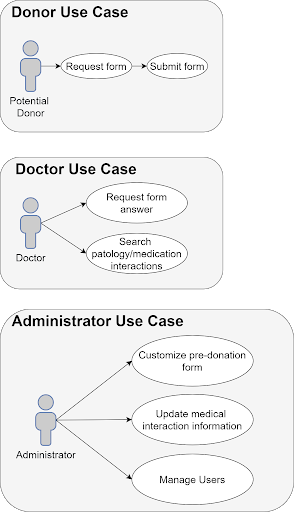
\includegraphics[trim={0 370 70 0},clip]{./figures/useCases.png}}
	\end{center}
	\caption{Donor use case.}\label{fig:donor_use_case}
\end{figure}

After a donor submits their form responses a doctor user will be able to access their answers by searching by the user's unique id as presented in Figure~\ref{fig:doctor_use_case}.

\begin{figure}[H]
	\begin{center}
		\resizebox{100mm}{!}{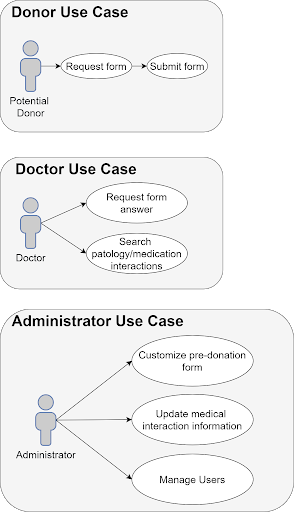
\includegraphics[trim={0 210 70 150},clip]{./figures/useCases.png}}
	\end{center}
	\caption{Doctor use case.}\label{fig:doctor_use_case}
\end{figure}

Furthermore the doctor user is able to search for pathology/medication interactions to resolve any inquiries that might appear during the screening.

Finally the administrator user can update the form structure and flow, update the interaction information and manage the platform's users.
The administrator use case is presented in Figure ~\ref{fig:administrator_use_case}.

\begin{figure}[H]
	\begin{center}
		\resizebox{100mm}{!}{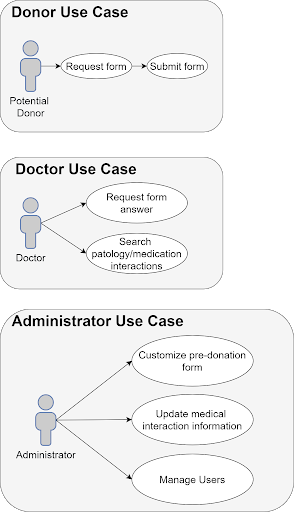
\includegraphics[trim={0 0 0 300},clip]{./figures/useCases.png}}
	\end{center}
	\caption{Administrator use case.}\label{fig:administrator_use_case}
\end{figure}

% Capitulo 3
%
% Capítulo 4
%
\chapter{Architecture} \label{cap:architecture}

This chapter provides an overview of the system’s components and their interactions.
It outlines the capabilities of the project and presents the architecture, entities, and
implementation blueprint that have been designed and developed.

\section{Overview}

Figure ~\ref{fig:architecture} presents a diagram illustrating the main components of the system and their interactions. The system consists of a backend application (server-side) and a frontend application (client-side).
The backend architecture consists of routes, services, and repositories. The routes handle incoming HTTP requests and call the appropriate service. The services manage data manipulation, validation, and interactions with external APIs or databases. Finally, the processed data is sent to the repositories, which store it in the database.

\begin{figure}[H]
	\begin{center}
		\resizebox{160mm}{!}{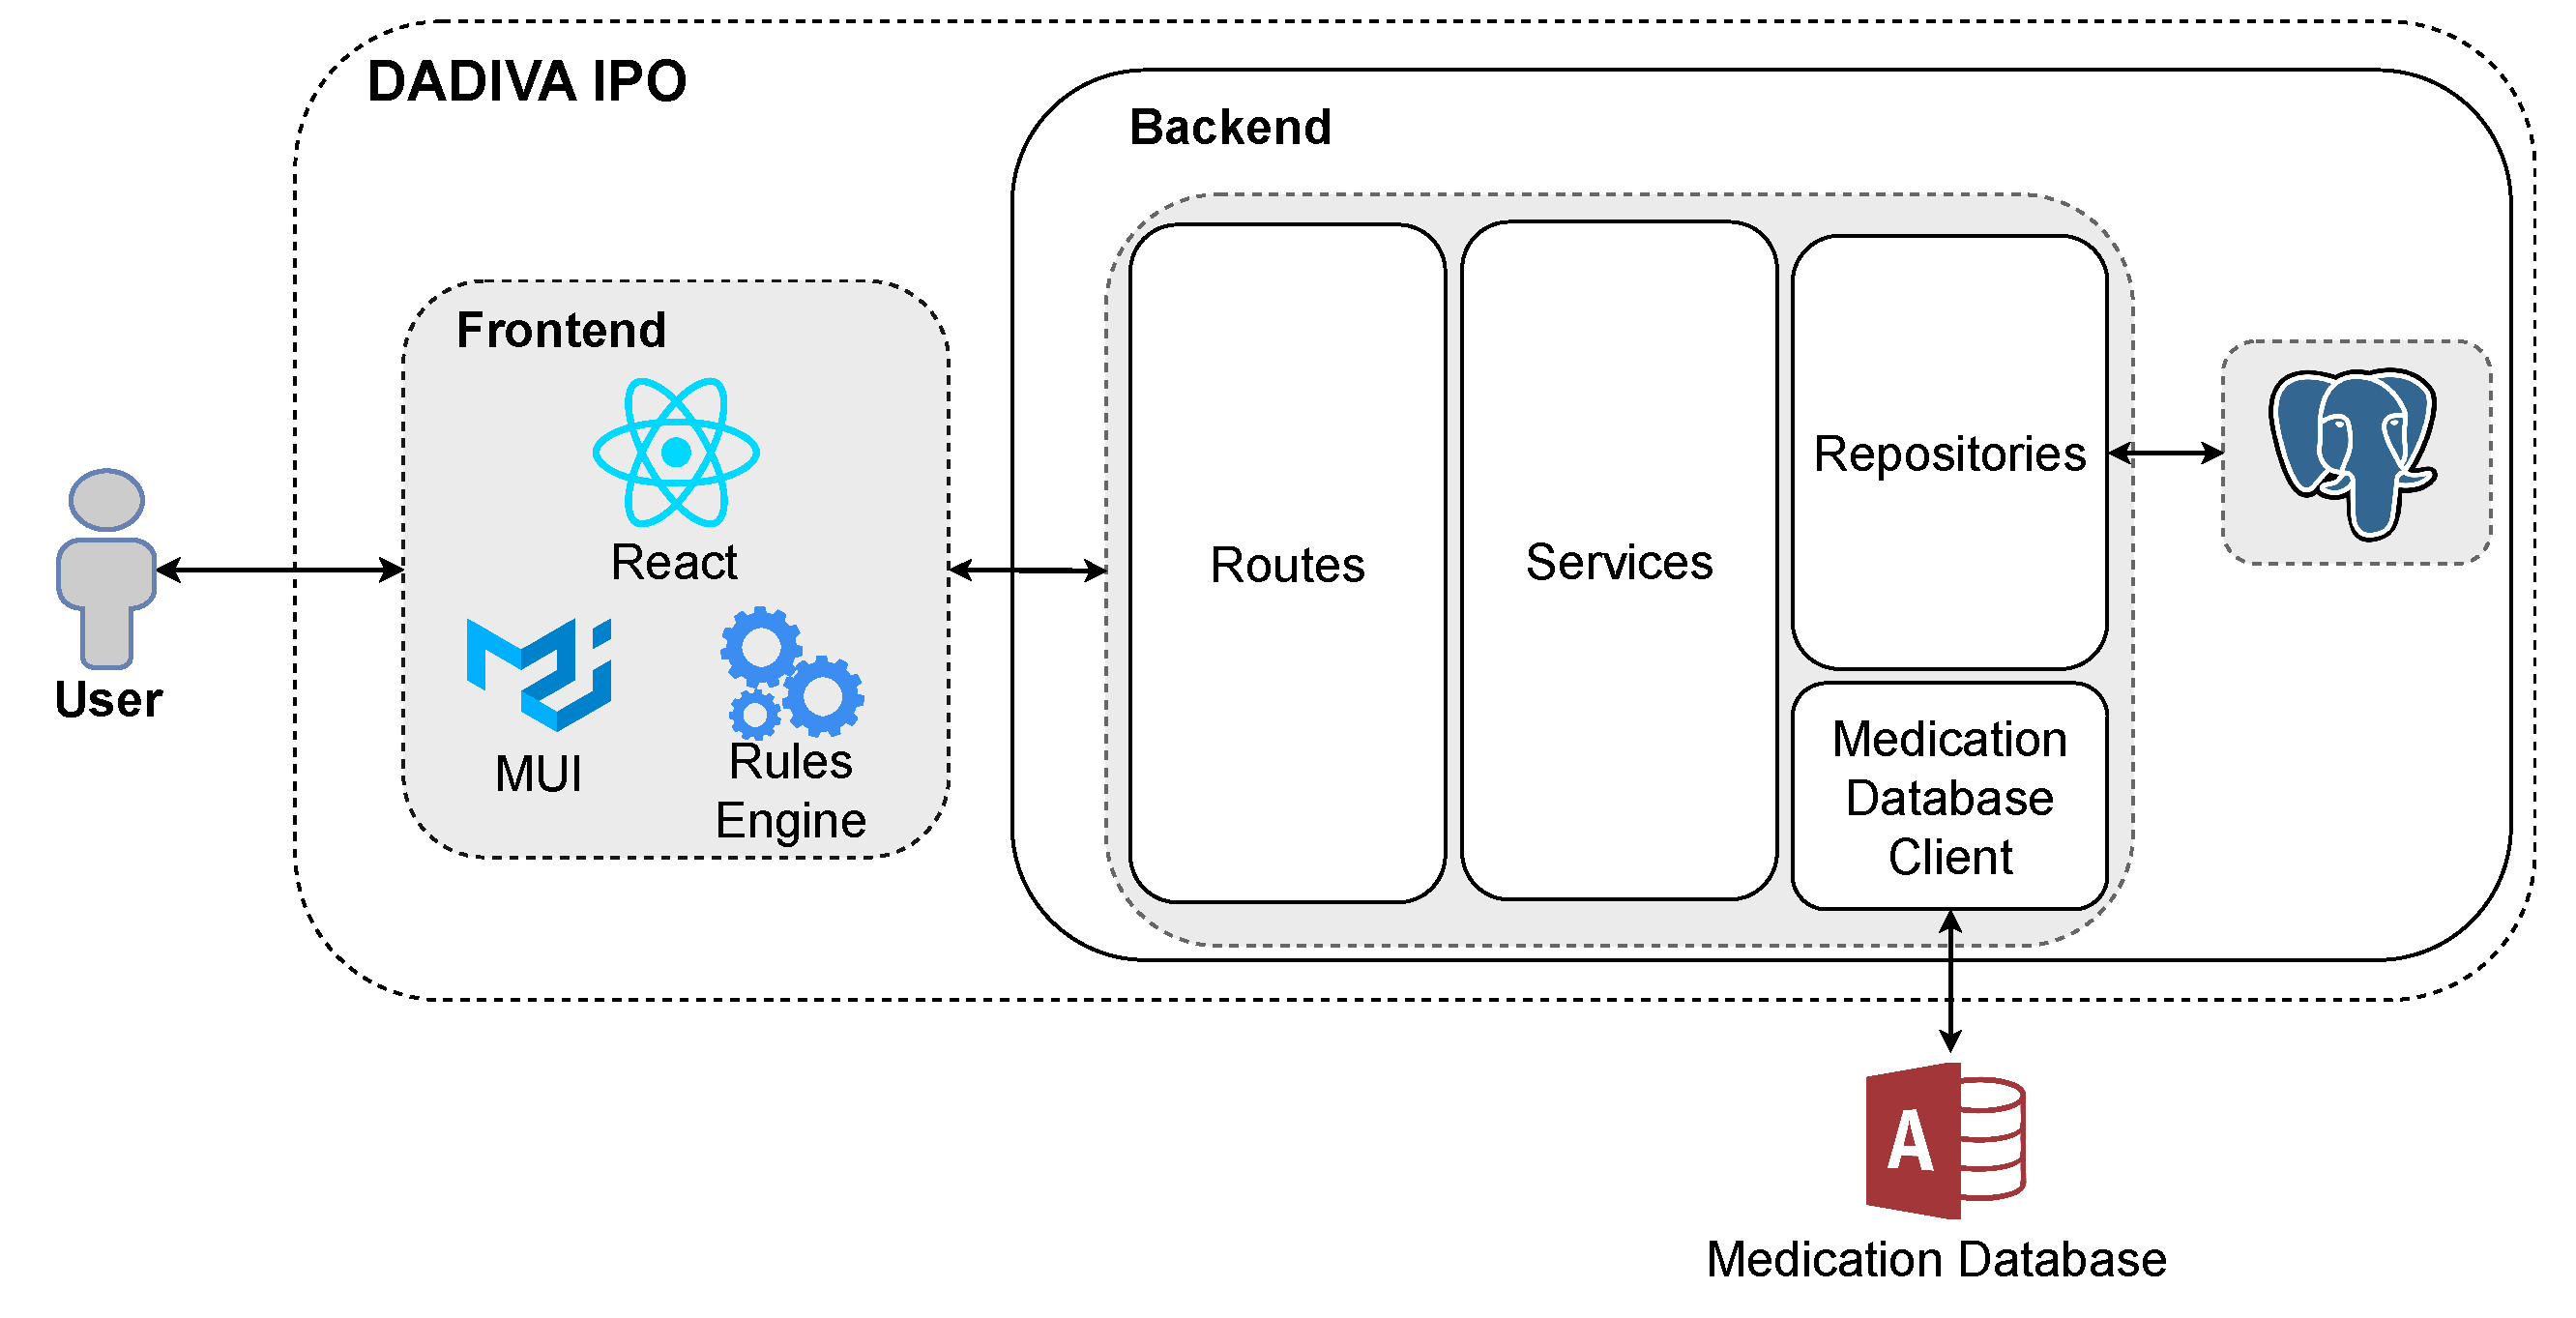
\includegraphics{./figures/Architecture.pdf}}
	\end{center}
	\caption{Application Architecture, gray squares represent containerized components of the solution.}\label{fig:architecture}
\end{figure}

\section{Backend Application}

The backend application can be abstracted into 3 layers:
\begin{itemize}
	\item routes: responsible for receiving the http request and calling the correct service;
	\item services: contains the services that manage the business logic of the application;
	\item repositories: contains the repository layer of the application, uses the ElasticSearchClient;
\end{itemize}


%The backend handles HTTP requests directed to specific endpoints. The route associated with each endpoint converts the request body into an appropriate model, if necessary, and then calls the corresponding service, passing along the model. The service validates the model, converts it into a domain object, and calls the relevant repository. Using an ElasticClient, the repository stores the object in the ElasticSearch database. The appropriate response is then propagated back up, as illustrated in Figure ~\ref{fig:backendLayers}.
%
%\begin{figure}[H]
%	\begin{center}
%		\resizebox{100mm}{!}{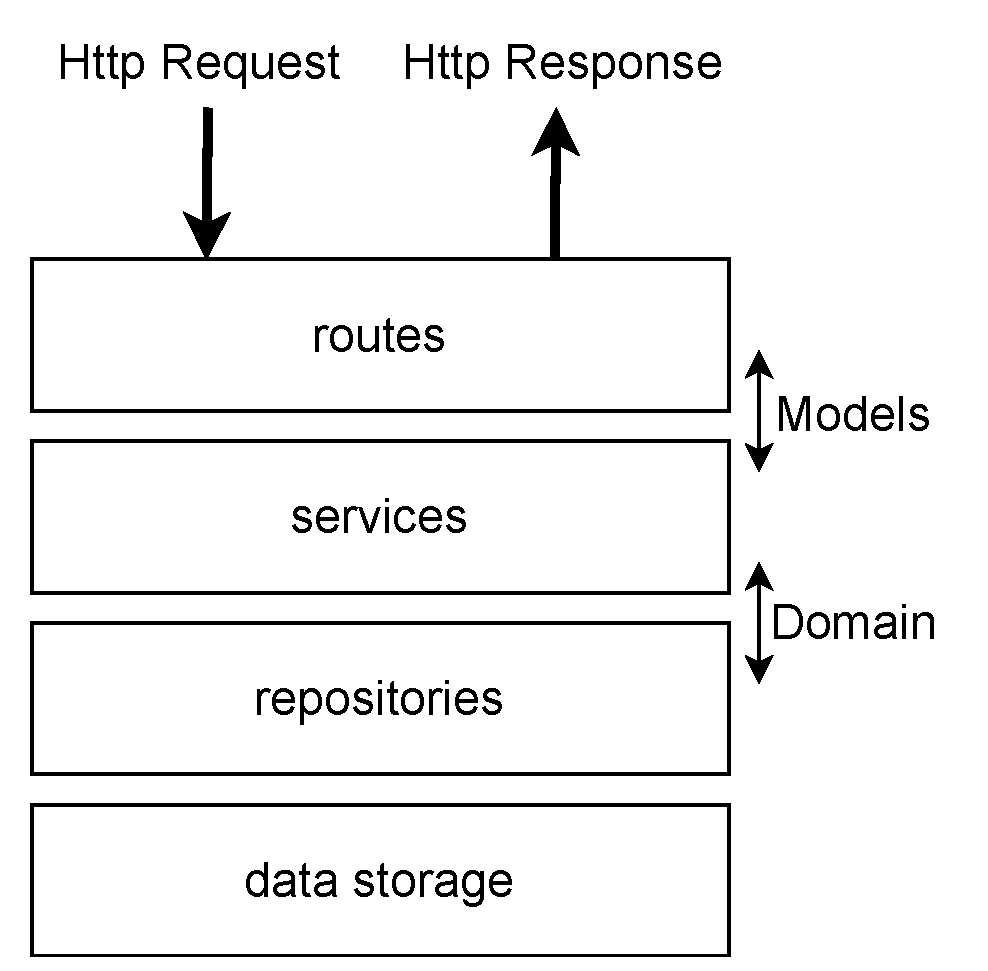
\includegraphics{./figures/backendLayers.pdf}}
%	\end{center}
%	\caption{Backend layers.}\label{fig:backendLayers}
%\end{figure}

The service layer is composed by the following elements:

\begin{itemize}
	\item form: responsible for form management, such as, creation, requests, submission, editing and deletion;
	\item search: responsible for medication and pathology interaction information retrieval;
	\item users: responsible for user management, such as, registration, login, deletion and role management.
\end{itemize}

The repositories communicate with the database, in which the various data models are divided into specific indexes, such as:

\begin{itemize}
	\item /form: stores all the form structures;
	\item /submissions: stores all the user form responses;
	\item /inconsistencies: stores all the user form inconsistencies;
	\item /users: stores all the users.
\end{itemize}

An example of a GET request for the form resource is presented in Figure ~\ref{fig:getForm_Sequence_Diagram}

\begin{figure}[H]
	\begin{center}
		\resizebox{160mm}{!}{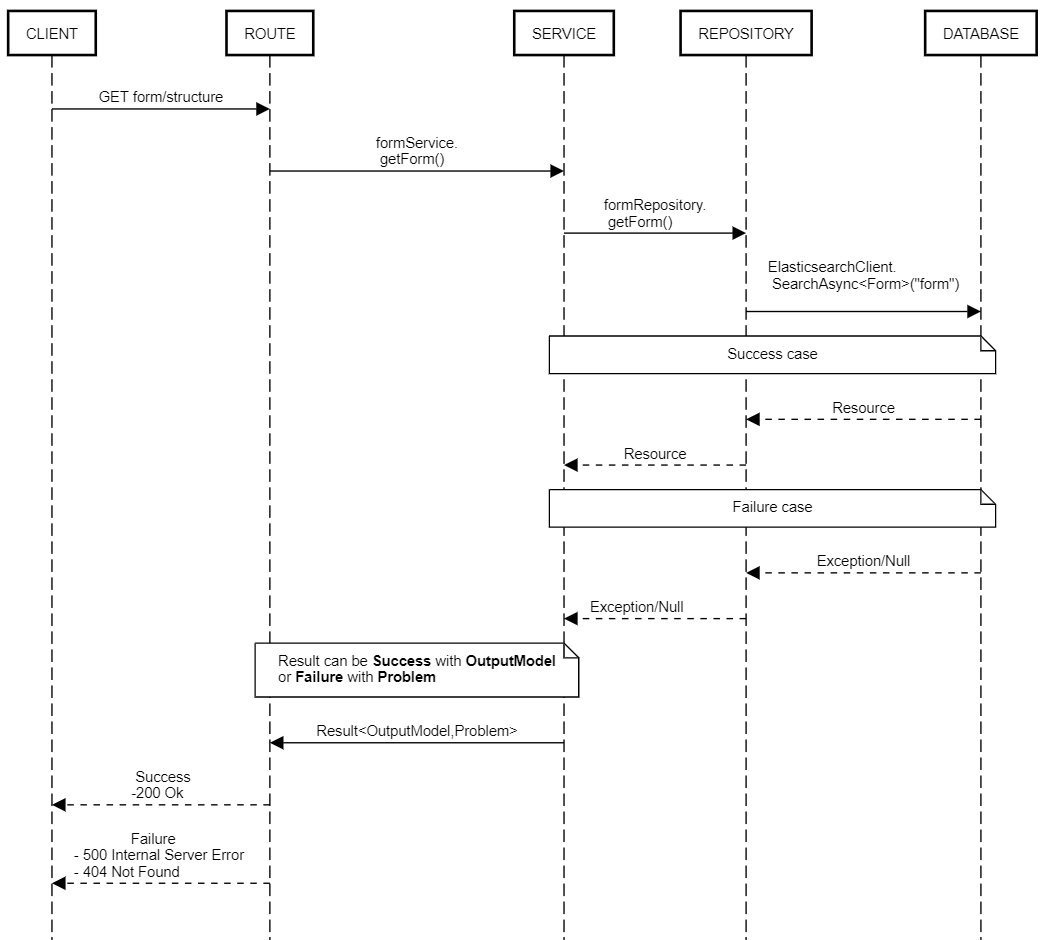
\includegraphics{./figures/getForm_Sequence_Diagram.png}}
	\end{center}
	\caption{Get Form Sequence Diagram.}\label{fig:getForm_Sequence_Diagram}
\end{figure}


\section{Form Data Model and Inconsistencies Data Model}

The first approach to solve the dynamic form challenge was to use a data structure formed by pairs of main questions and sub-questions, example presented in Figure ~\ref{fig:old_form}, where a main question can only be answered with boolean values, and one of those values triggers the display of a sub-question which has a certain type of response, such as boolean, dropdown for known multiple answers, and text, to accept user text input.

\begin{figure}[hbt!]
	\begin{center}
		\resizebox{150mm}{!}{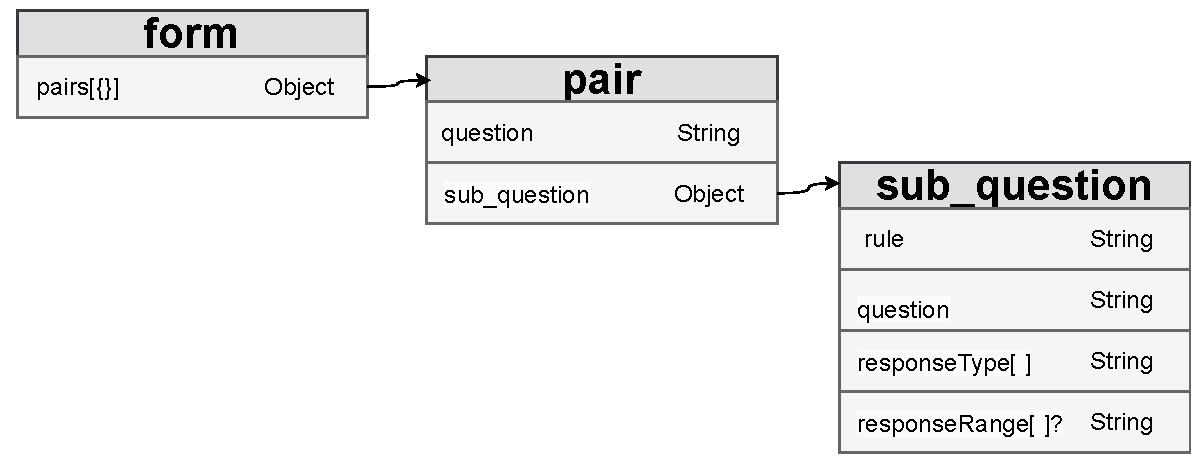
\includegraphics{./figures/oldForm.pdf}}
	\end{center}
	\caption{First Form Data Structure.}\label{fig:old_form}
\end{figure}

This approach has several drawbacks. Firstly, it prevents the suppression of further questions, which contradicts the goal of creating a flexible and adaptable solution. Additionally, it conflates questions and rules within sub-questions, leading to a lack of clarity and potential confusion in implementation.

Upon further discussion we settled on using a more complex data structure , exemplified in Figure ~\ref{fig:new_form}, composed by a list of questions and a list of rules.

Each question has an id, the text that composes it, the type of response (boolean, text and dropdown) and can have options that lists all the possibles values for a multiple(dropdown) response.

Each rule has conditions, which can be "any","all" or "not", so that, when any, all or none of the conditions are met an event is triggered.
Each condition type will have a fact, an operator and a value. In essence, when a question, which is identified by the fact field via it's id, is answered a condition can true or false depending on the logical operator used, ie equal or notEqual, and the value of the answer. If the condition is true an event is triggered, this event can be to show or hide a subsequent question, this targeted question is identified via the id, supplied in the params field.

This model, specifically the rules field, was chosen as it is part of the JSON-Rules-Engine specification, which is presented in more detail in Chapter ~\ref{cap:technologies} and is easily stored and retrieved in a ElasticSearch database.

\begin{figure}[htbp]
	\begin{center}
		{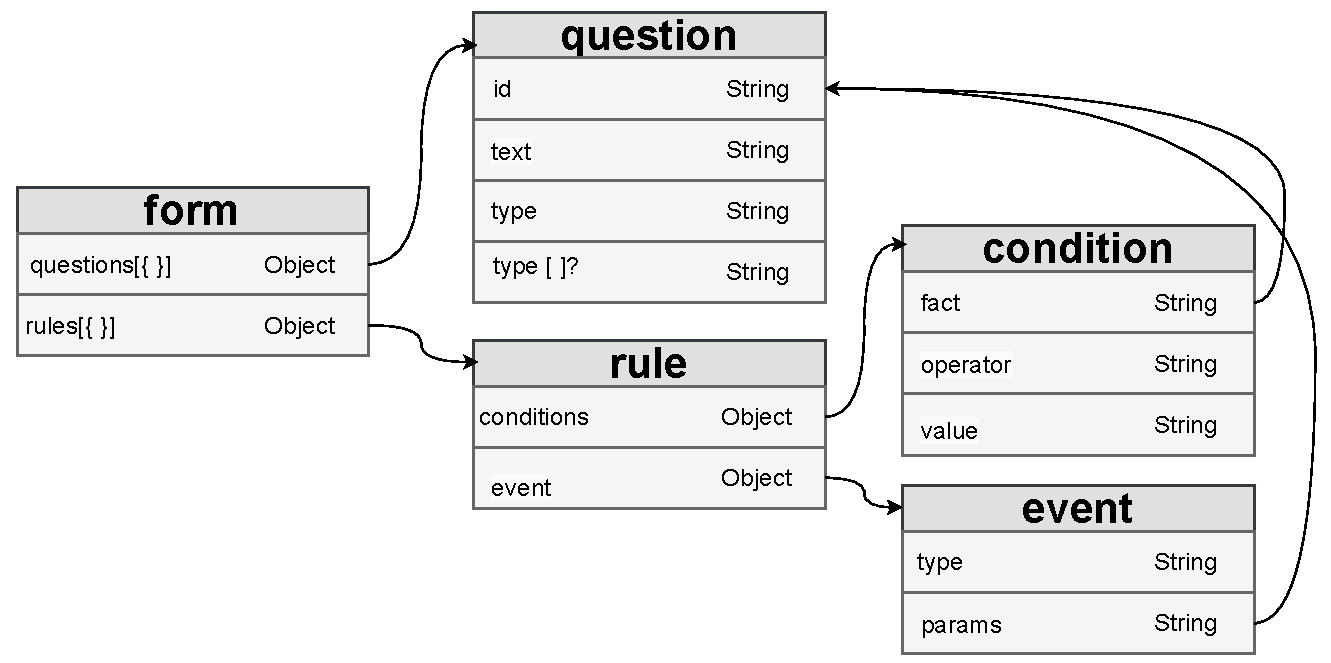
\includegraphics[width=\textwidth,height=\textheight,keepaspectratio]{./figures/newForm.pdf}}
	\end{center}
	\caption{Final Form Data Structure.}\label{fig:new_form}
\end{figure}
\FloatBarrier

The inconsistencies data model is compromised of rules, and describes answer combinations that are logical fallacies, ie a donor answering that they're healthy in one question and that they have a chronic disease in another question.

\section{Submission Data Model}

The submission data structure represents and answered form, has such it contains a list of answered questions, each answered question is composed by the question id and the answer, as referenced in Figure ~\ref{fig:submission_data_model}.

\begin{figure}[hbt!]
	\begin{center}
		\resizebox{150mm}{!}{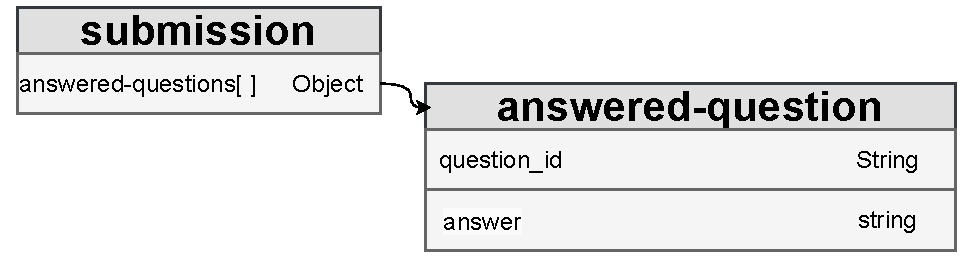
\includegraphics{./figures/Submission_Data_Model.pdf}}
	\end{center}
	\caption{Submission Data Structure.}\label{fig:submission_data_model}
\end{figure}


\section{User Data Model}

The user data structure is composed on an unique identifier, the nic, and the user hashed password, as referenced in Figure ~\ref{fig:user_data_model}.

\begin{figure}[hbt!]
	\begin{center}
		\resizebox{150mm}{!}{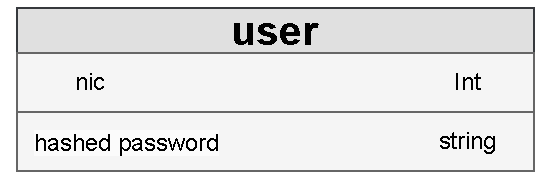
\includegraphics{./figures/User_Data_Structure.pdf}}
	\end{center}
	\caption{User Data Structure.}\label{fig:user_data_model}
\end{figure}

%%secalhar é mais adequado na descrição do problema
\section{IPO Medication Portal}
\textcolor{red}{
The IPST medication guideline are organized in a table like manner, in the following column layout:
	\begin{enumerate}
		\item Class/Group of Medication: This column categorizes medications.
		\item Active Substance/Commercial Name: This column lists either the active ingredient or the brand name of the medication.
		\item Criteria: This column specifies if a particular class or group of medications affects eligibility for blood donation, including details such as the duration of ineligibility and other relevant conditions.
	\end{enumerate}
	The terms used in the first column are, from what we can access, similar to the available pharmacotherapeutic classifications. A reliable source of a drug's pharmacotherapeutic classification is a portal provided by Infarmed to it's partner organizations, such as Lisbon's IPO.
	As such, upon a donor's form submission, assuming they where taking some medication, our application would perform requests to said portal, get the appropriate pharmacotherapeutic classification and, by cross-checking the classification with the term used in the first column of the guidelines, return the relevant information.
	However the terms used in the guidelines don't always reflect the available classifications, and, as such, the platform will employ a dictionary that associates the terms used in the guidelines to pharmacotherapeutic classifications. This dictionary will be updatable by the platform's administrators.
	The fact that the IPST guidelines aren't available in a machine readable format persists.
}

\section{Frontend Application}\label{architecture_frontend}

The frontend application is a web-based interface designed to facilitate seamless interaction between users and the backend system. It features a user-friendly and intuitive interface, catering to different types of users with specific functionalities:

\begin{itemize}
	\item Donor Users: Can fill out the current donation form;
	\item Doctor Users: Can search for pathology and medication interactions with blood donation and request form answers for specific users;
	\item Administrator Users: Can customize the current form, update pathology and medication interaction information, and manage users.
\end{itemize}

The application is organized into multiple pages and components, each serving distinct purposes. It includes a service layer responsible for communicating with the backend application through the REST API.

During planning some mockups where created of the final result for some pages, the login page is presented in Figure ~\ref{fig:login}, the form pages are presented in Figures ~\ref{fig:form},~\ref{fig:form_no} and ~\ref{fig:form_yes}, the backoffice page is presented in Figure ~\ref{fig:backoffice}.

\begin{figure}[H]
	\begin{center}
		\resizebox{160mm}{!}{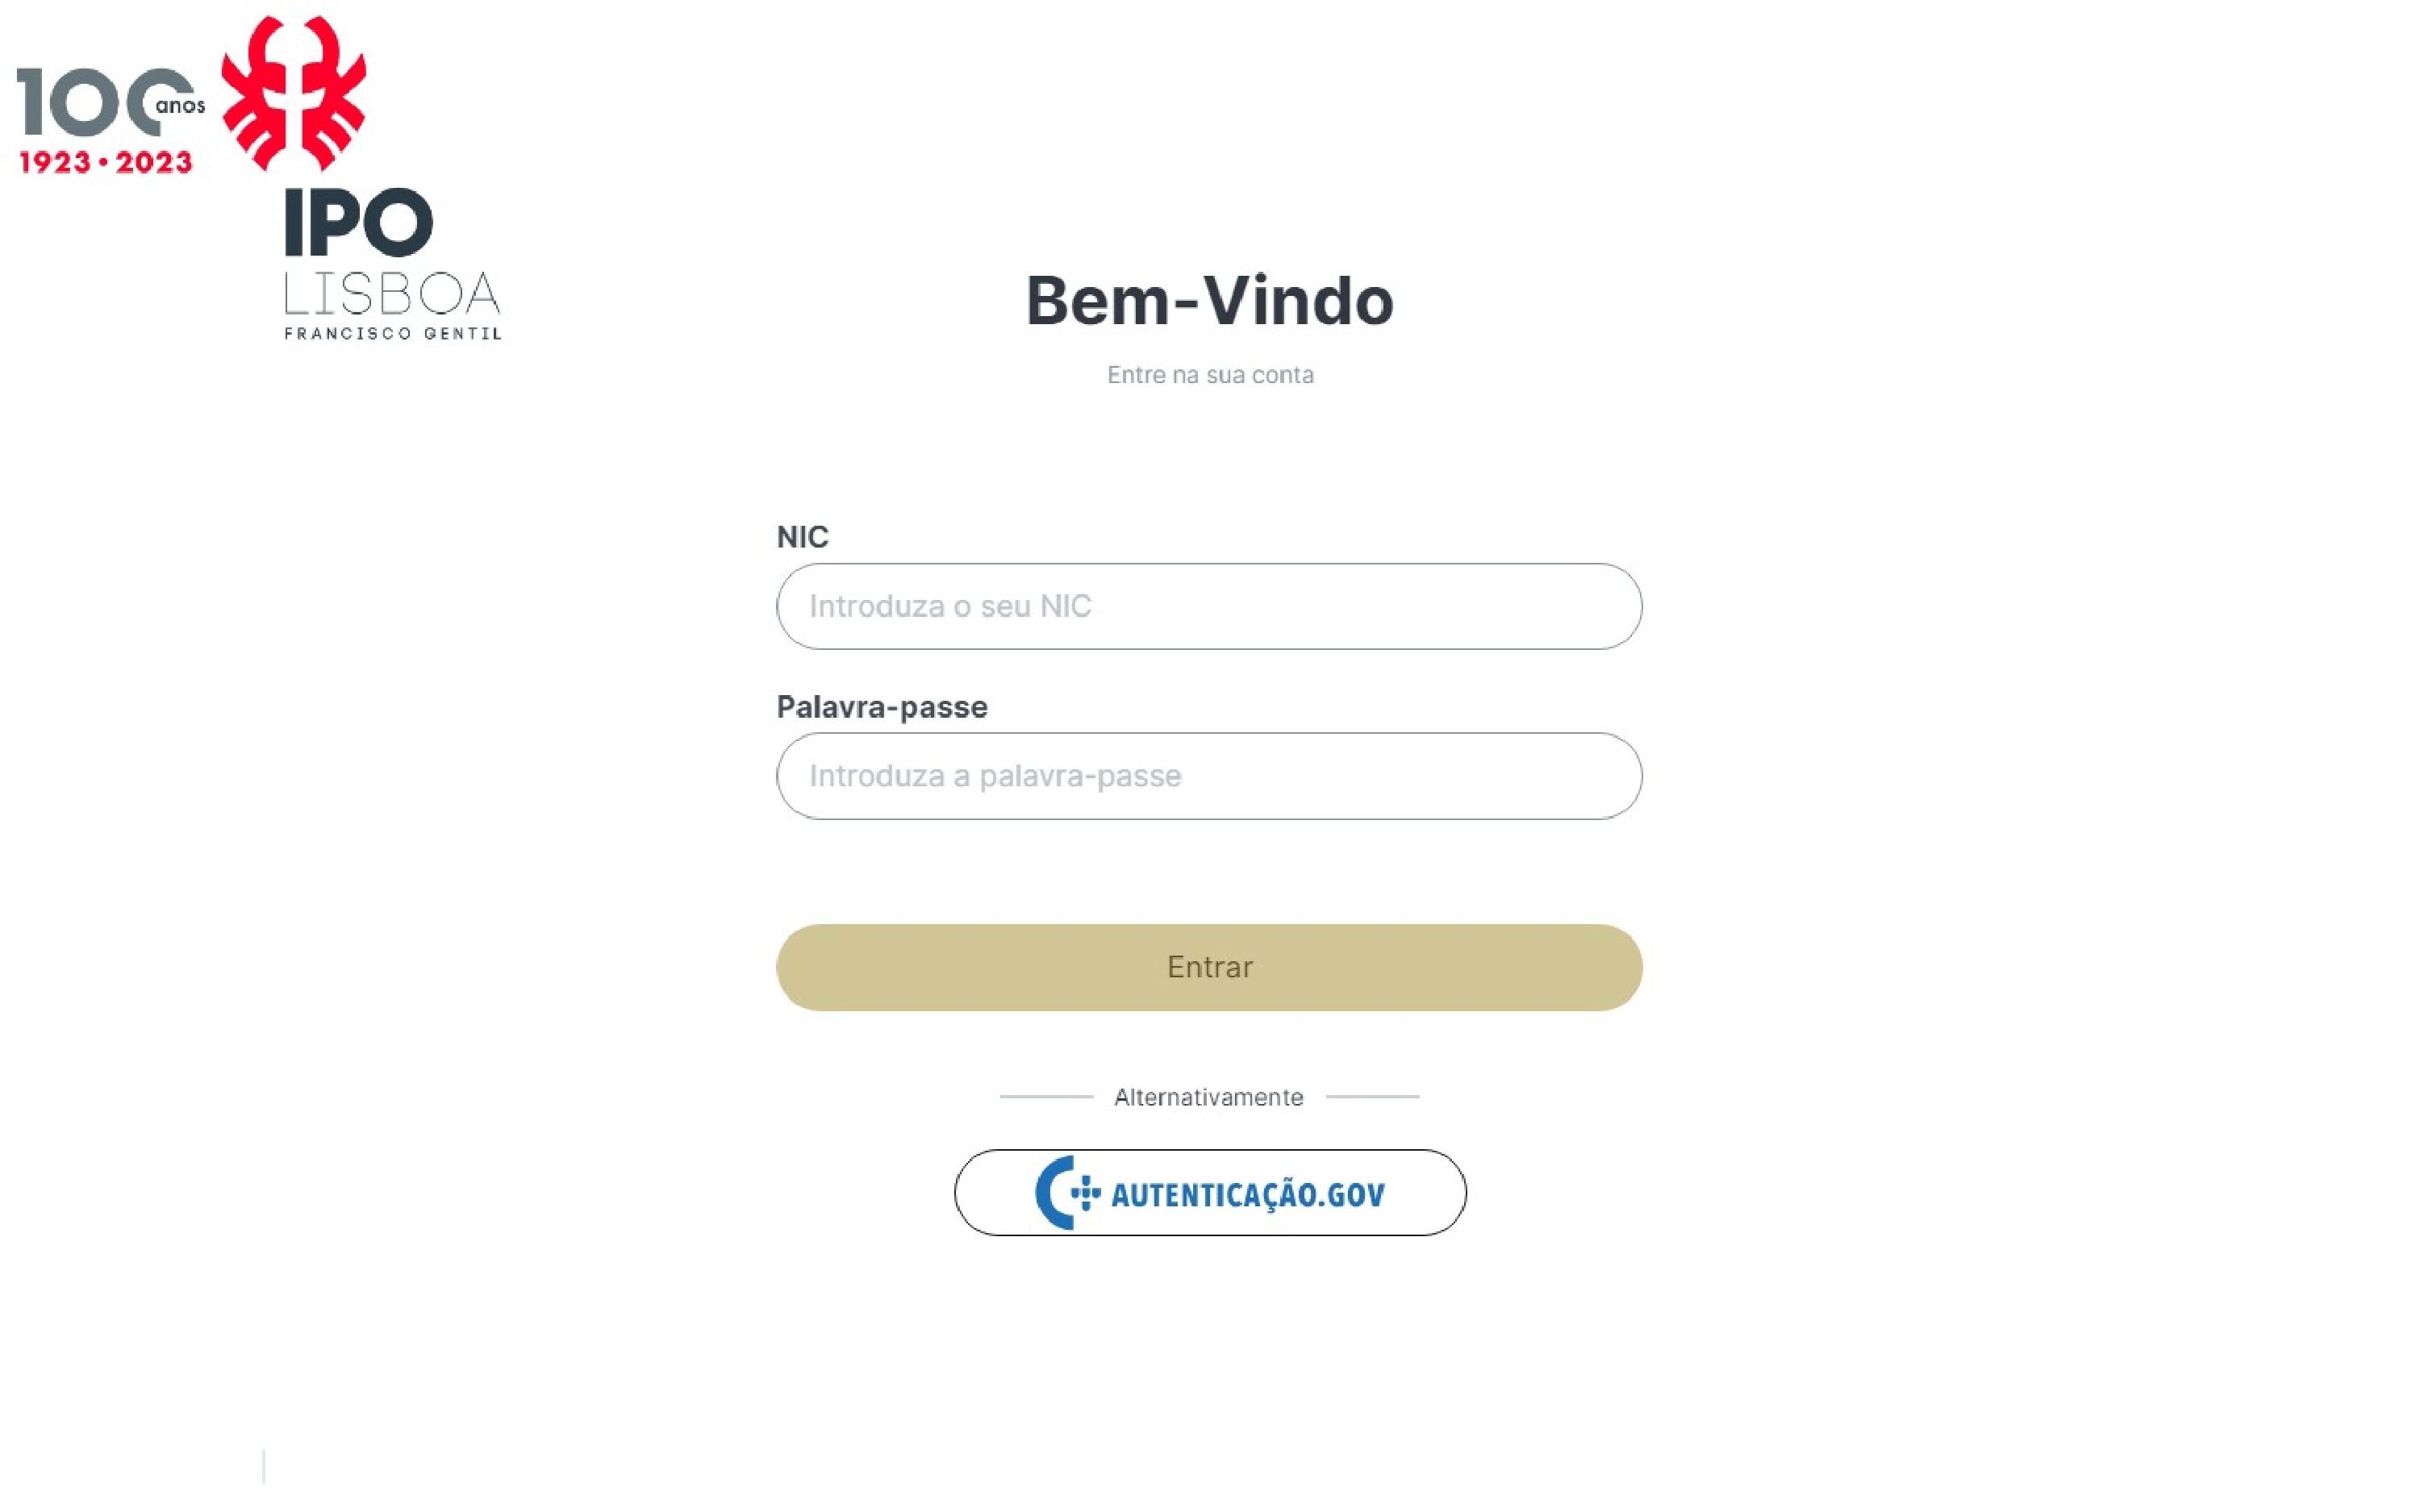
\includegraphics{./figures/Login.pdf}}
	\end{center}
	\caption{Login Page Mock.}\label{fig:login}
\end{figure}

\begin{figure}[H]
	\begin{center}
		\resizebox{160mm}{!}{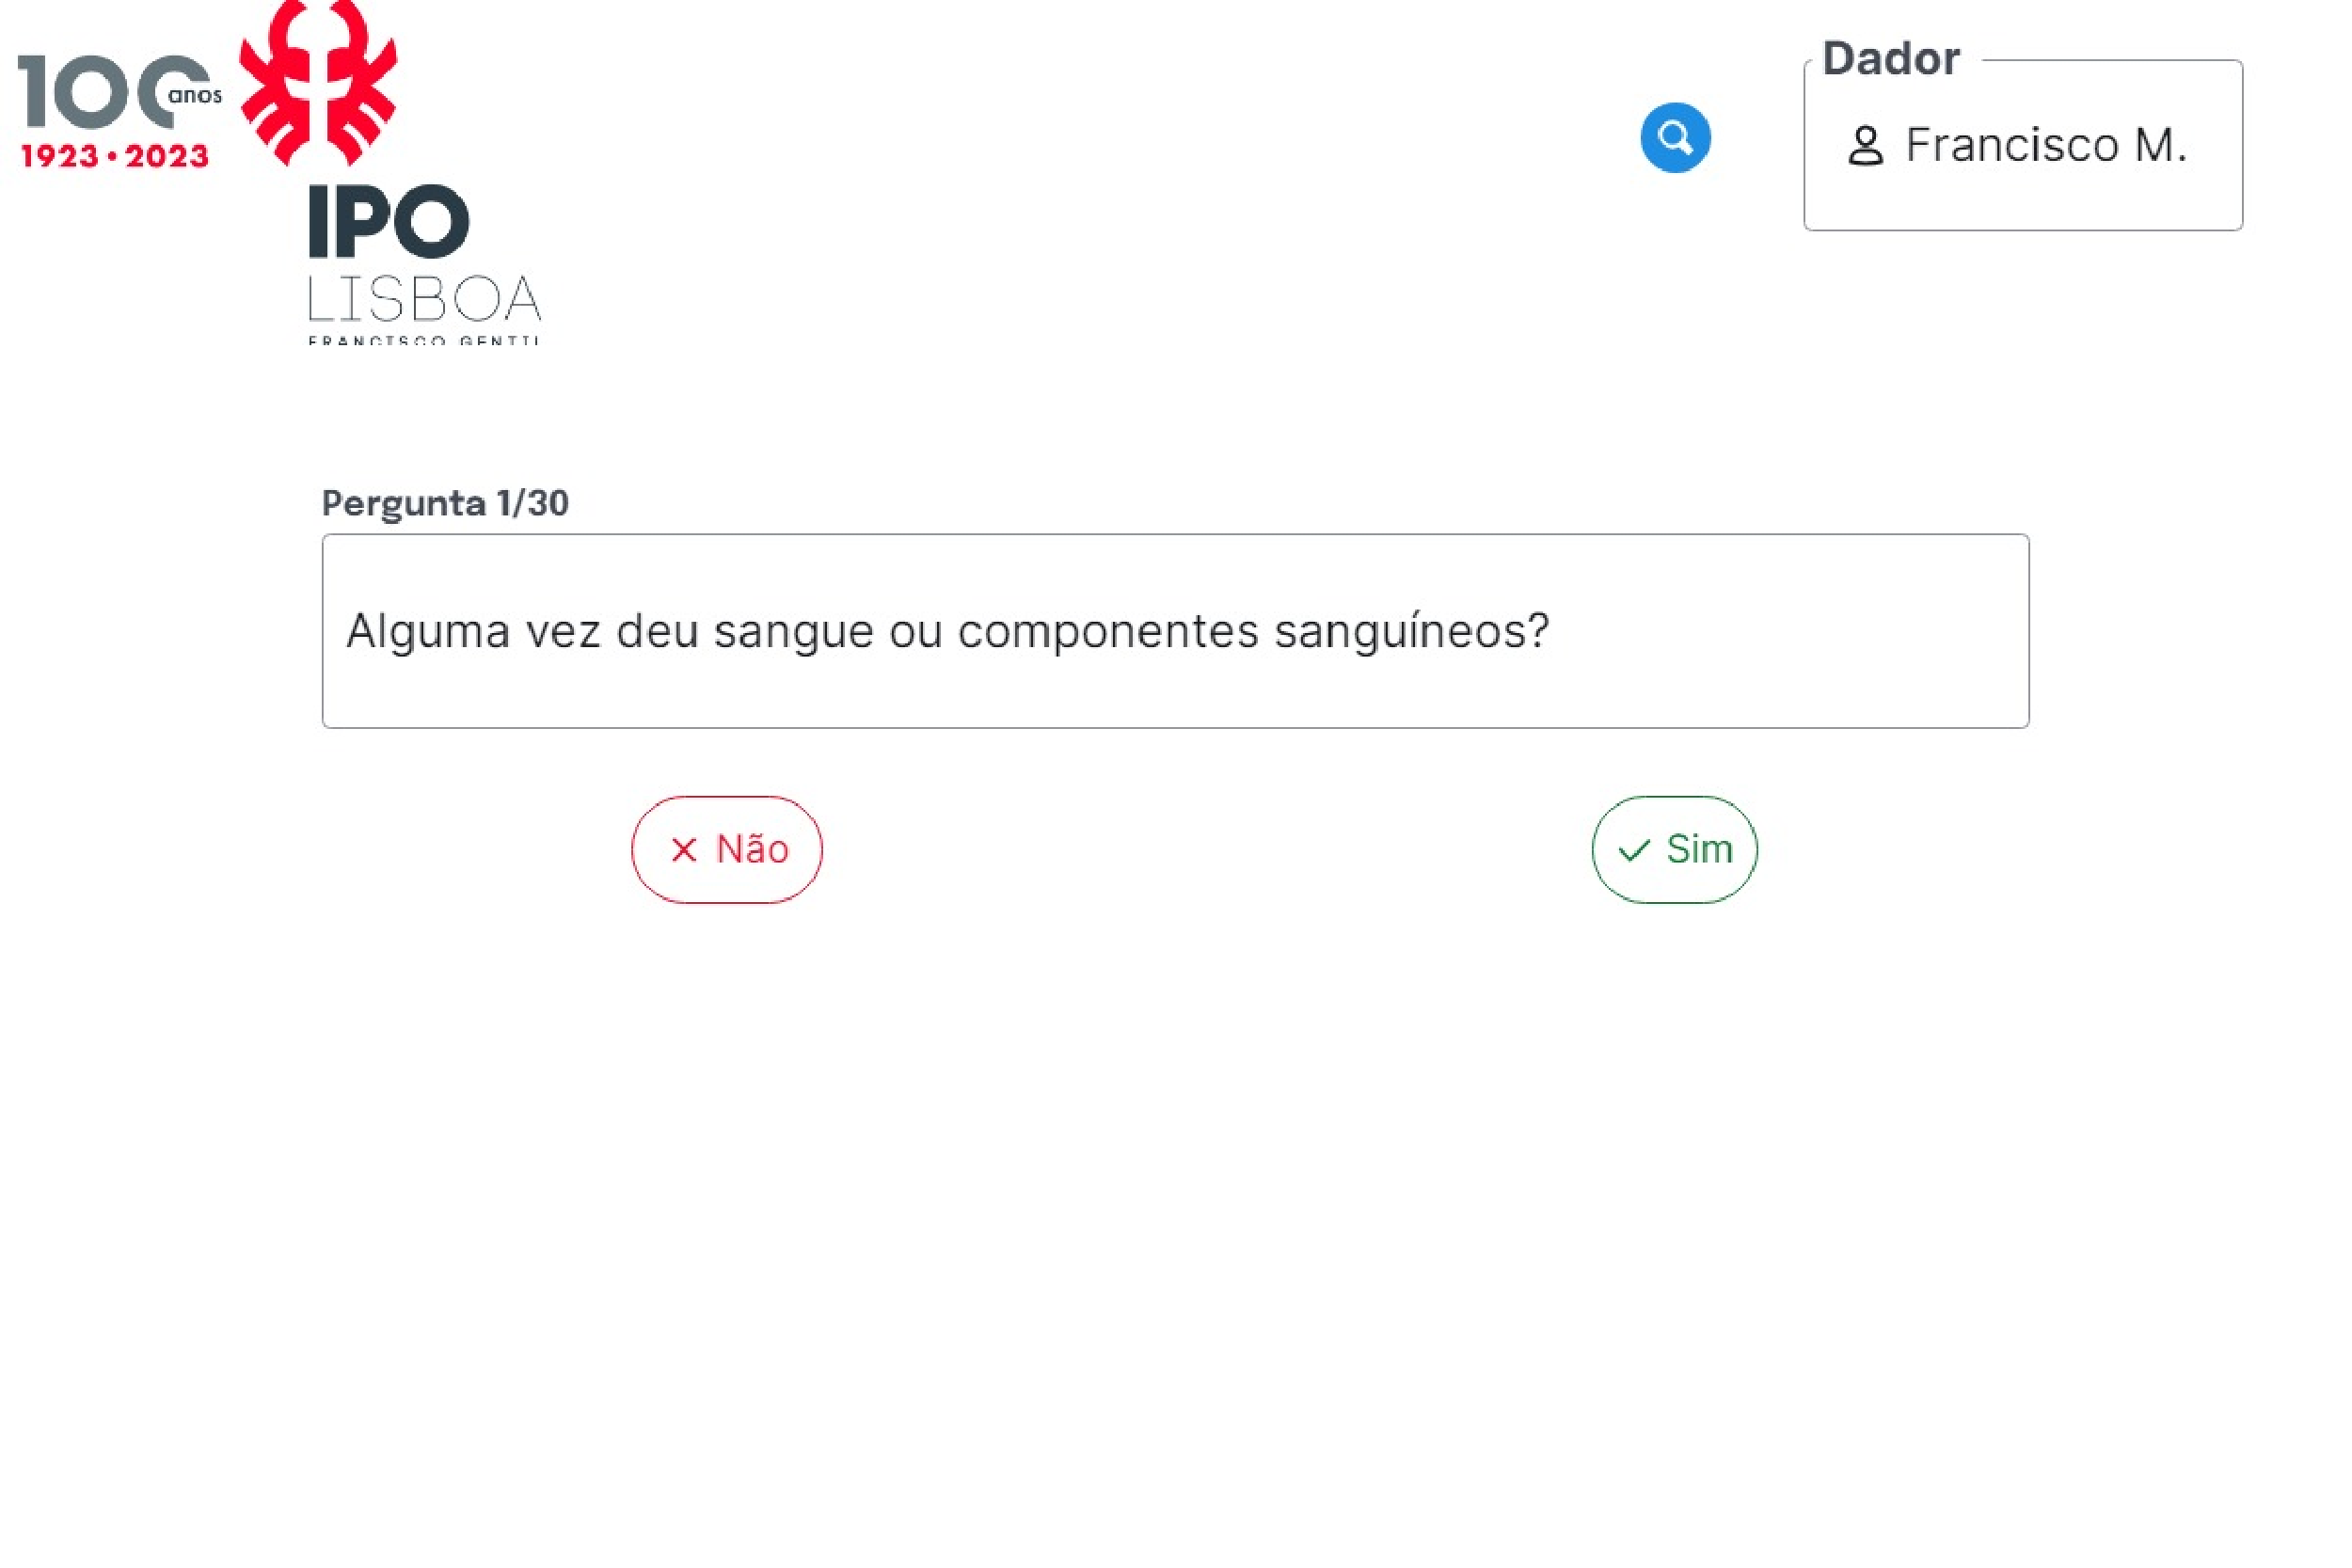
\includegraphics{./figures/Form.pdf}}
	\end{center}
	\caption{Form Page Mock.}\label{fig:form}
\end{figure}

\begin{figure}[H]
	\begin{center}
		\resizebox{160mm}{!}{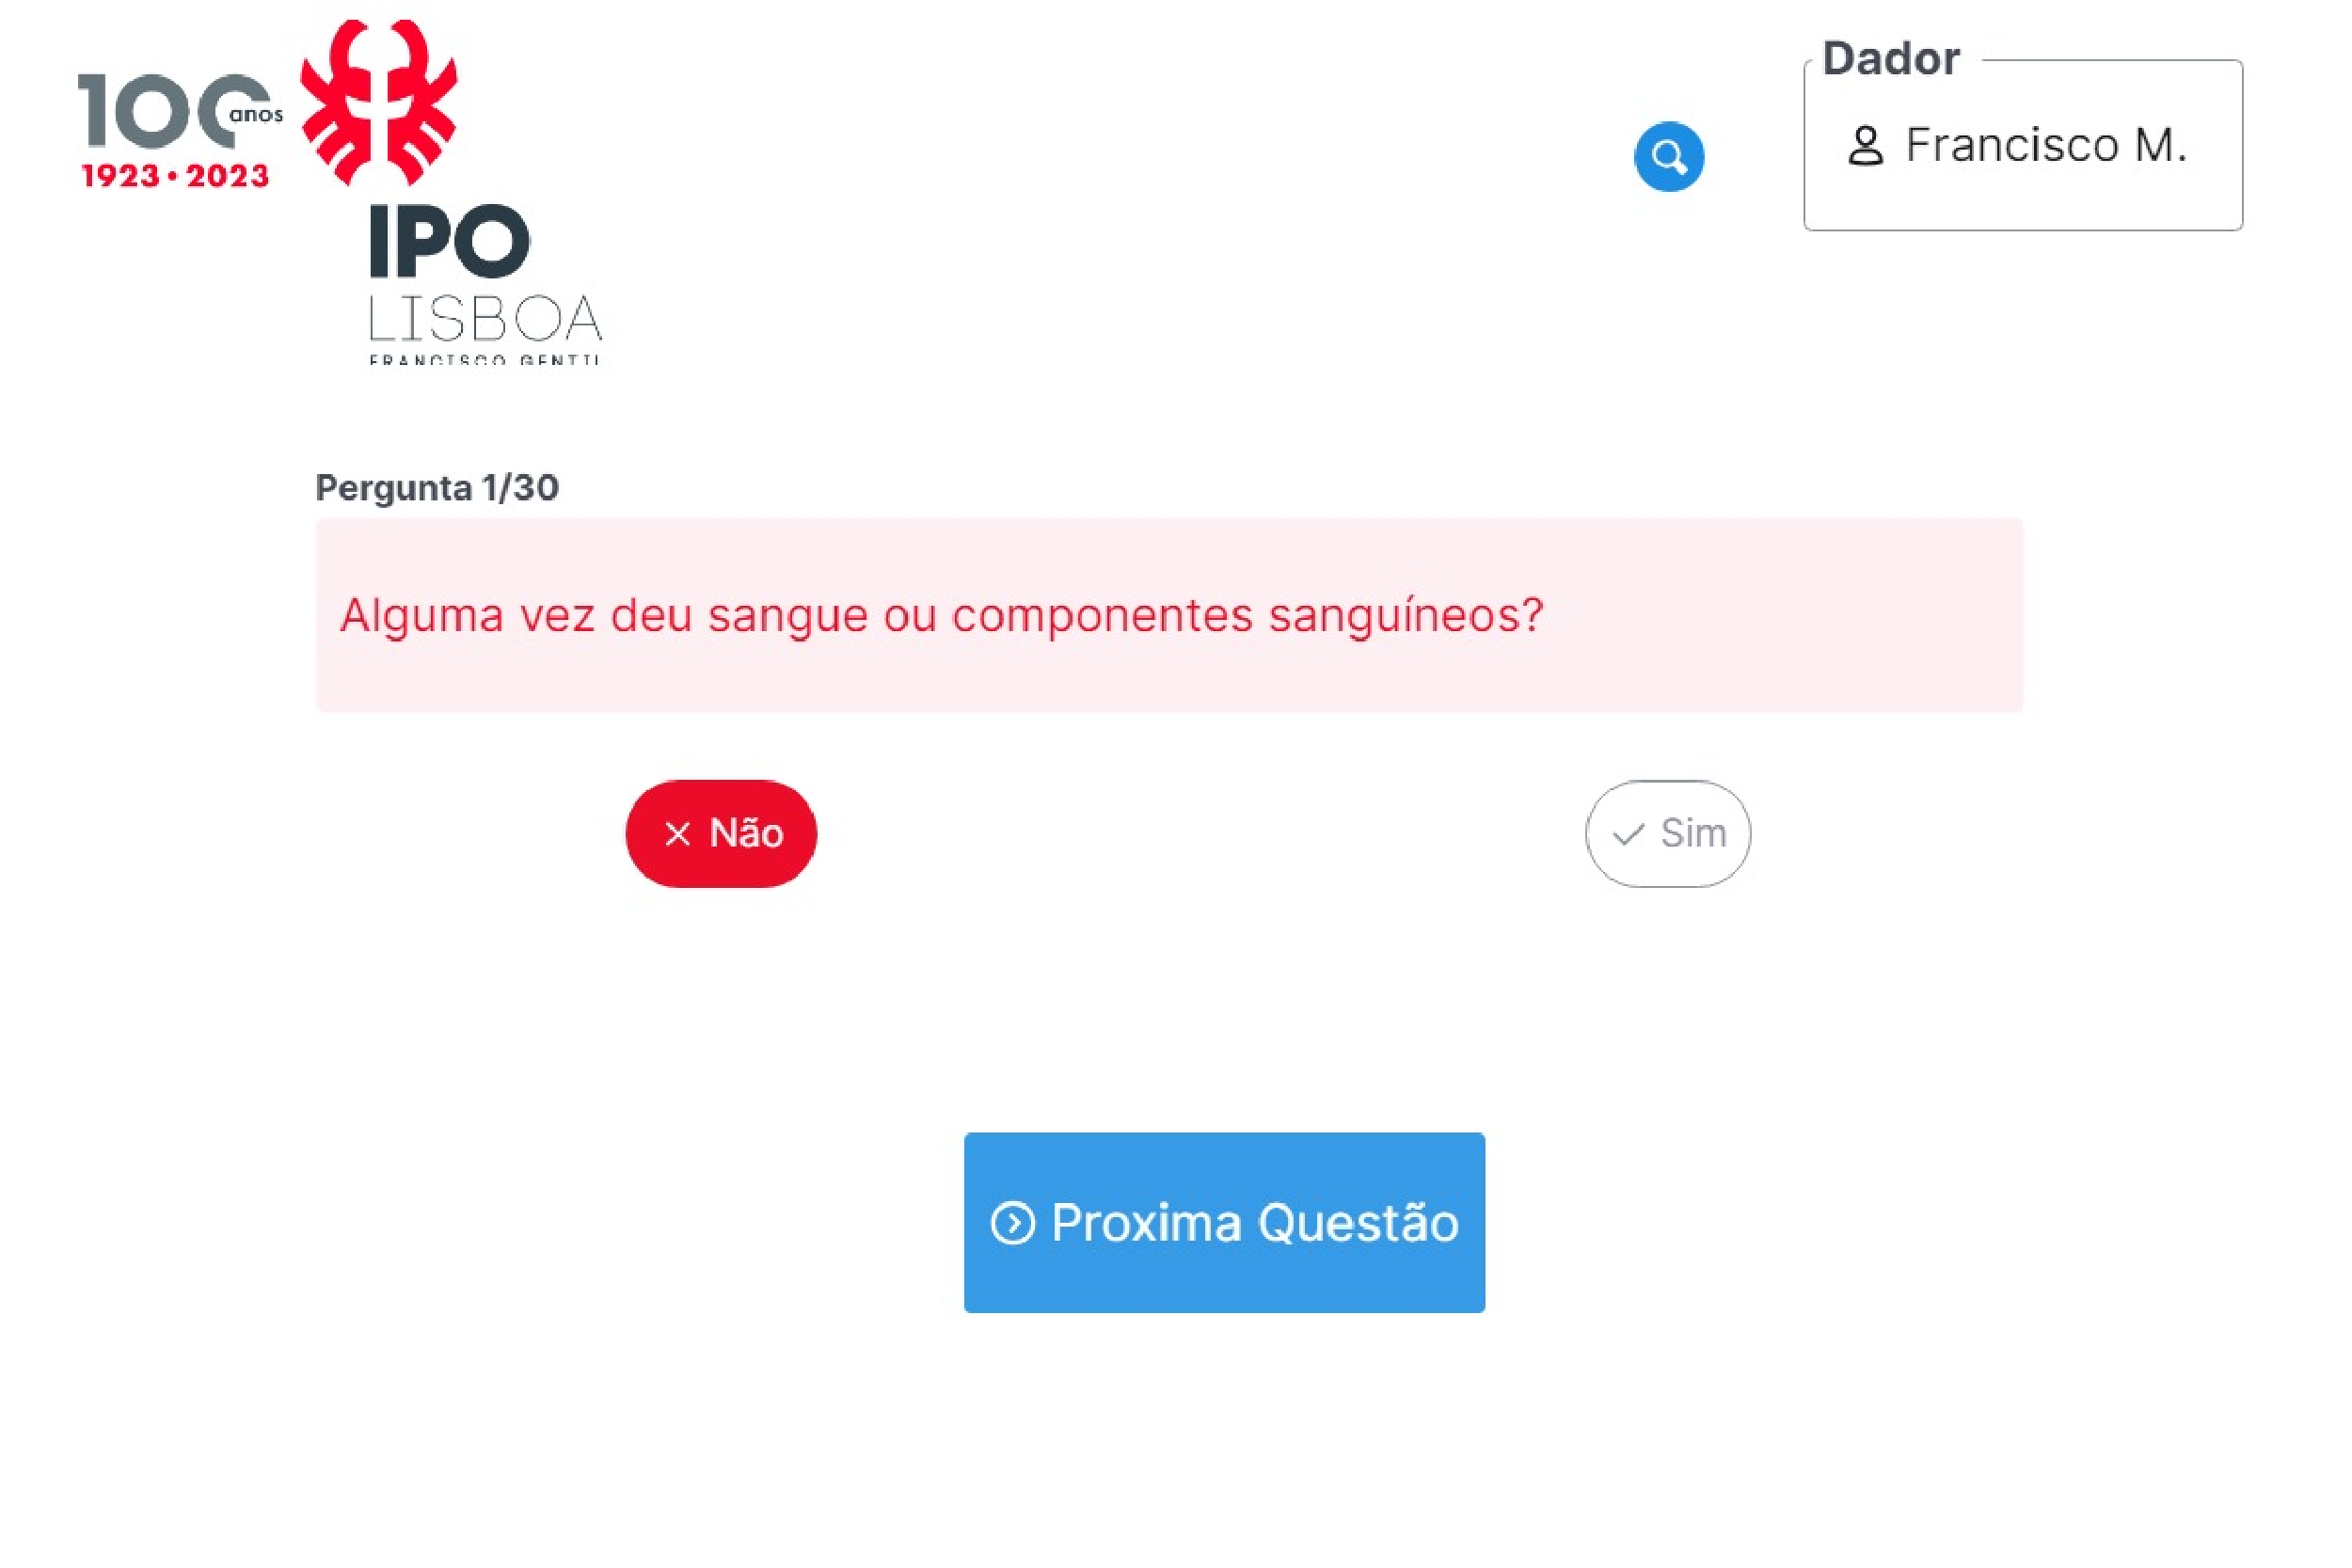
\includegraphics{./figures/Form_Answer_No.pdf}}
	\end{center}
	\caption{Form Page Negative Answer Mock.}\label{fig:form_no}
\end{figure}

\begin{figure}[H]
	\begin{center}
		\resizebox{160mm}{!}{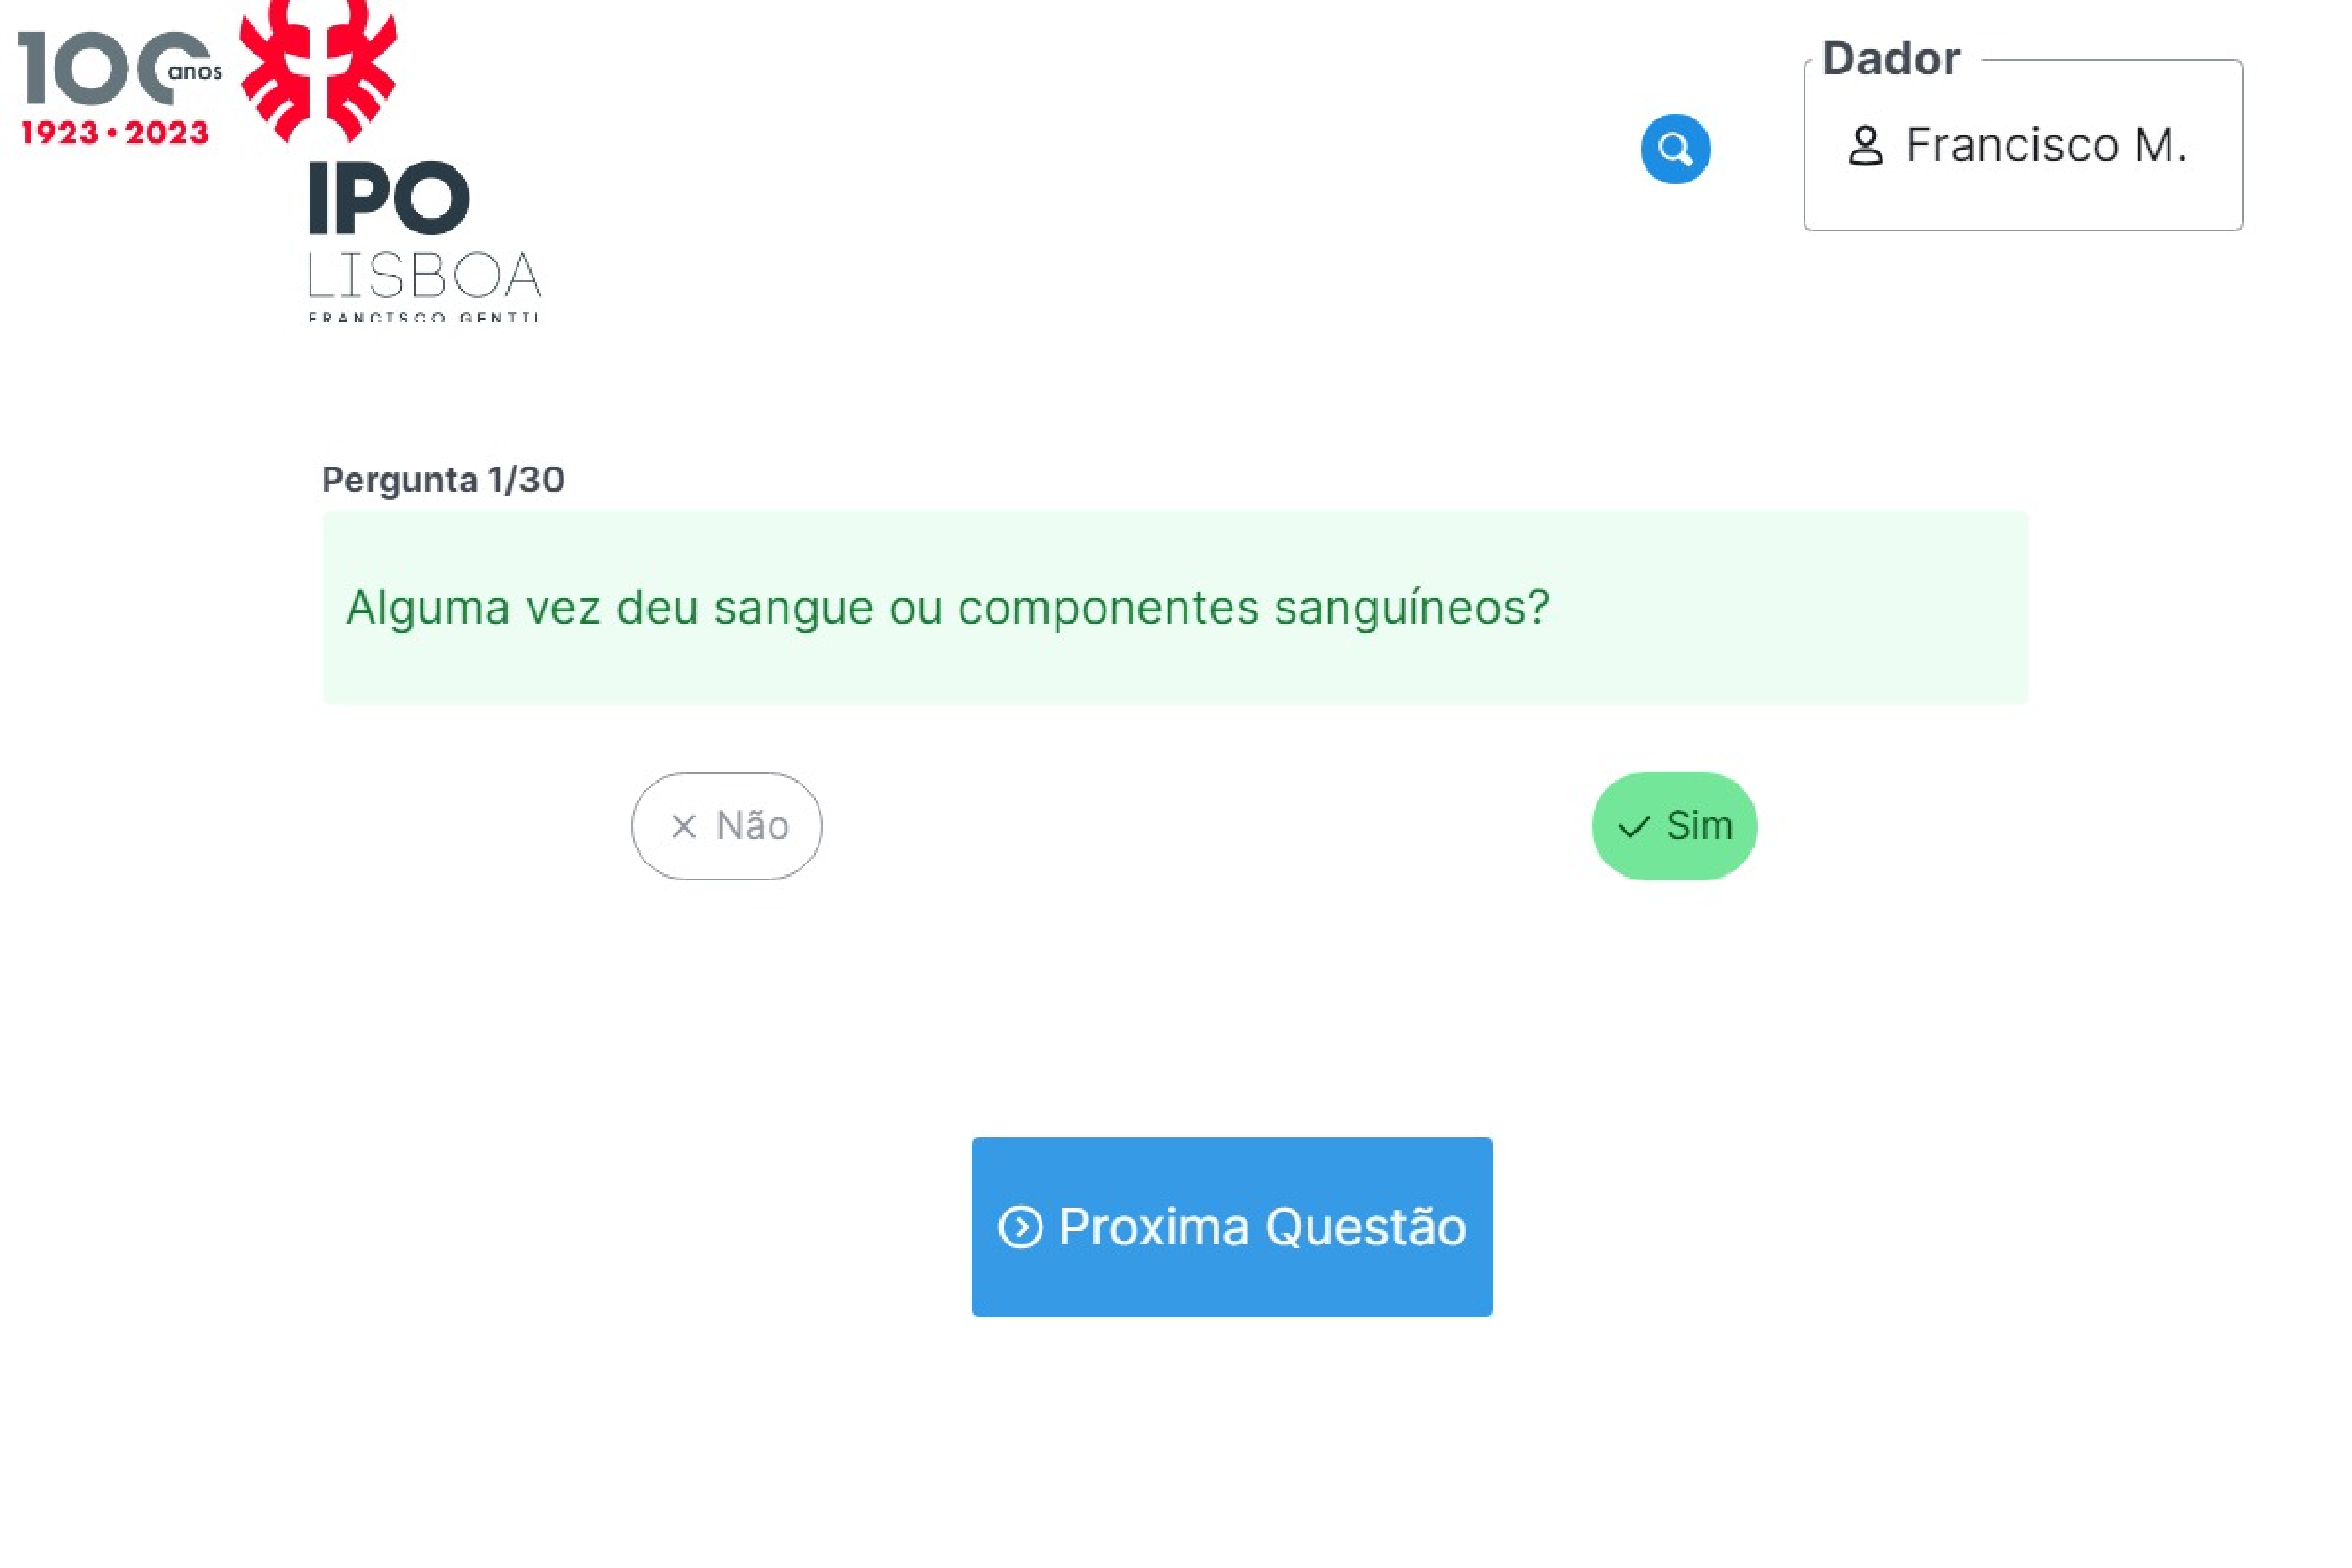
\includegraphics{./figures/Form_Answer_Yes.pdf}}
	\end{center}
	\caption{Form Page Positive Answer Mock.}\label{fig:form_yes}
\end{figure}

\begin{figure}[H]
	\begin{center}
		\resizebox{160mm}{!}{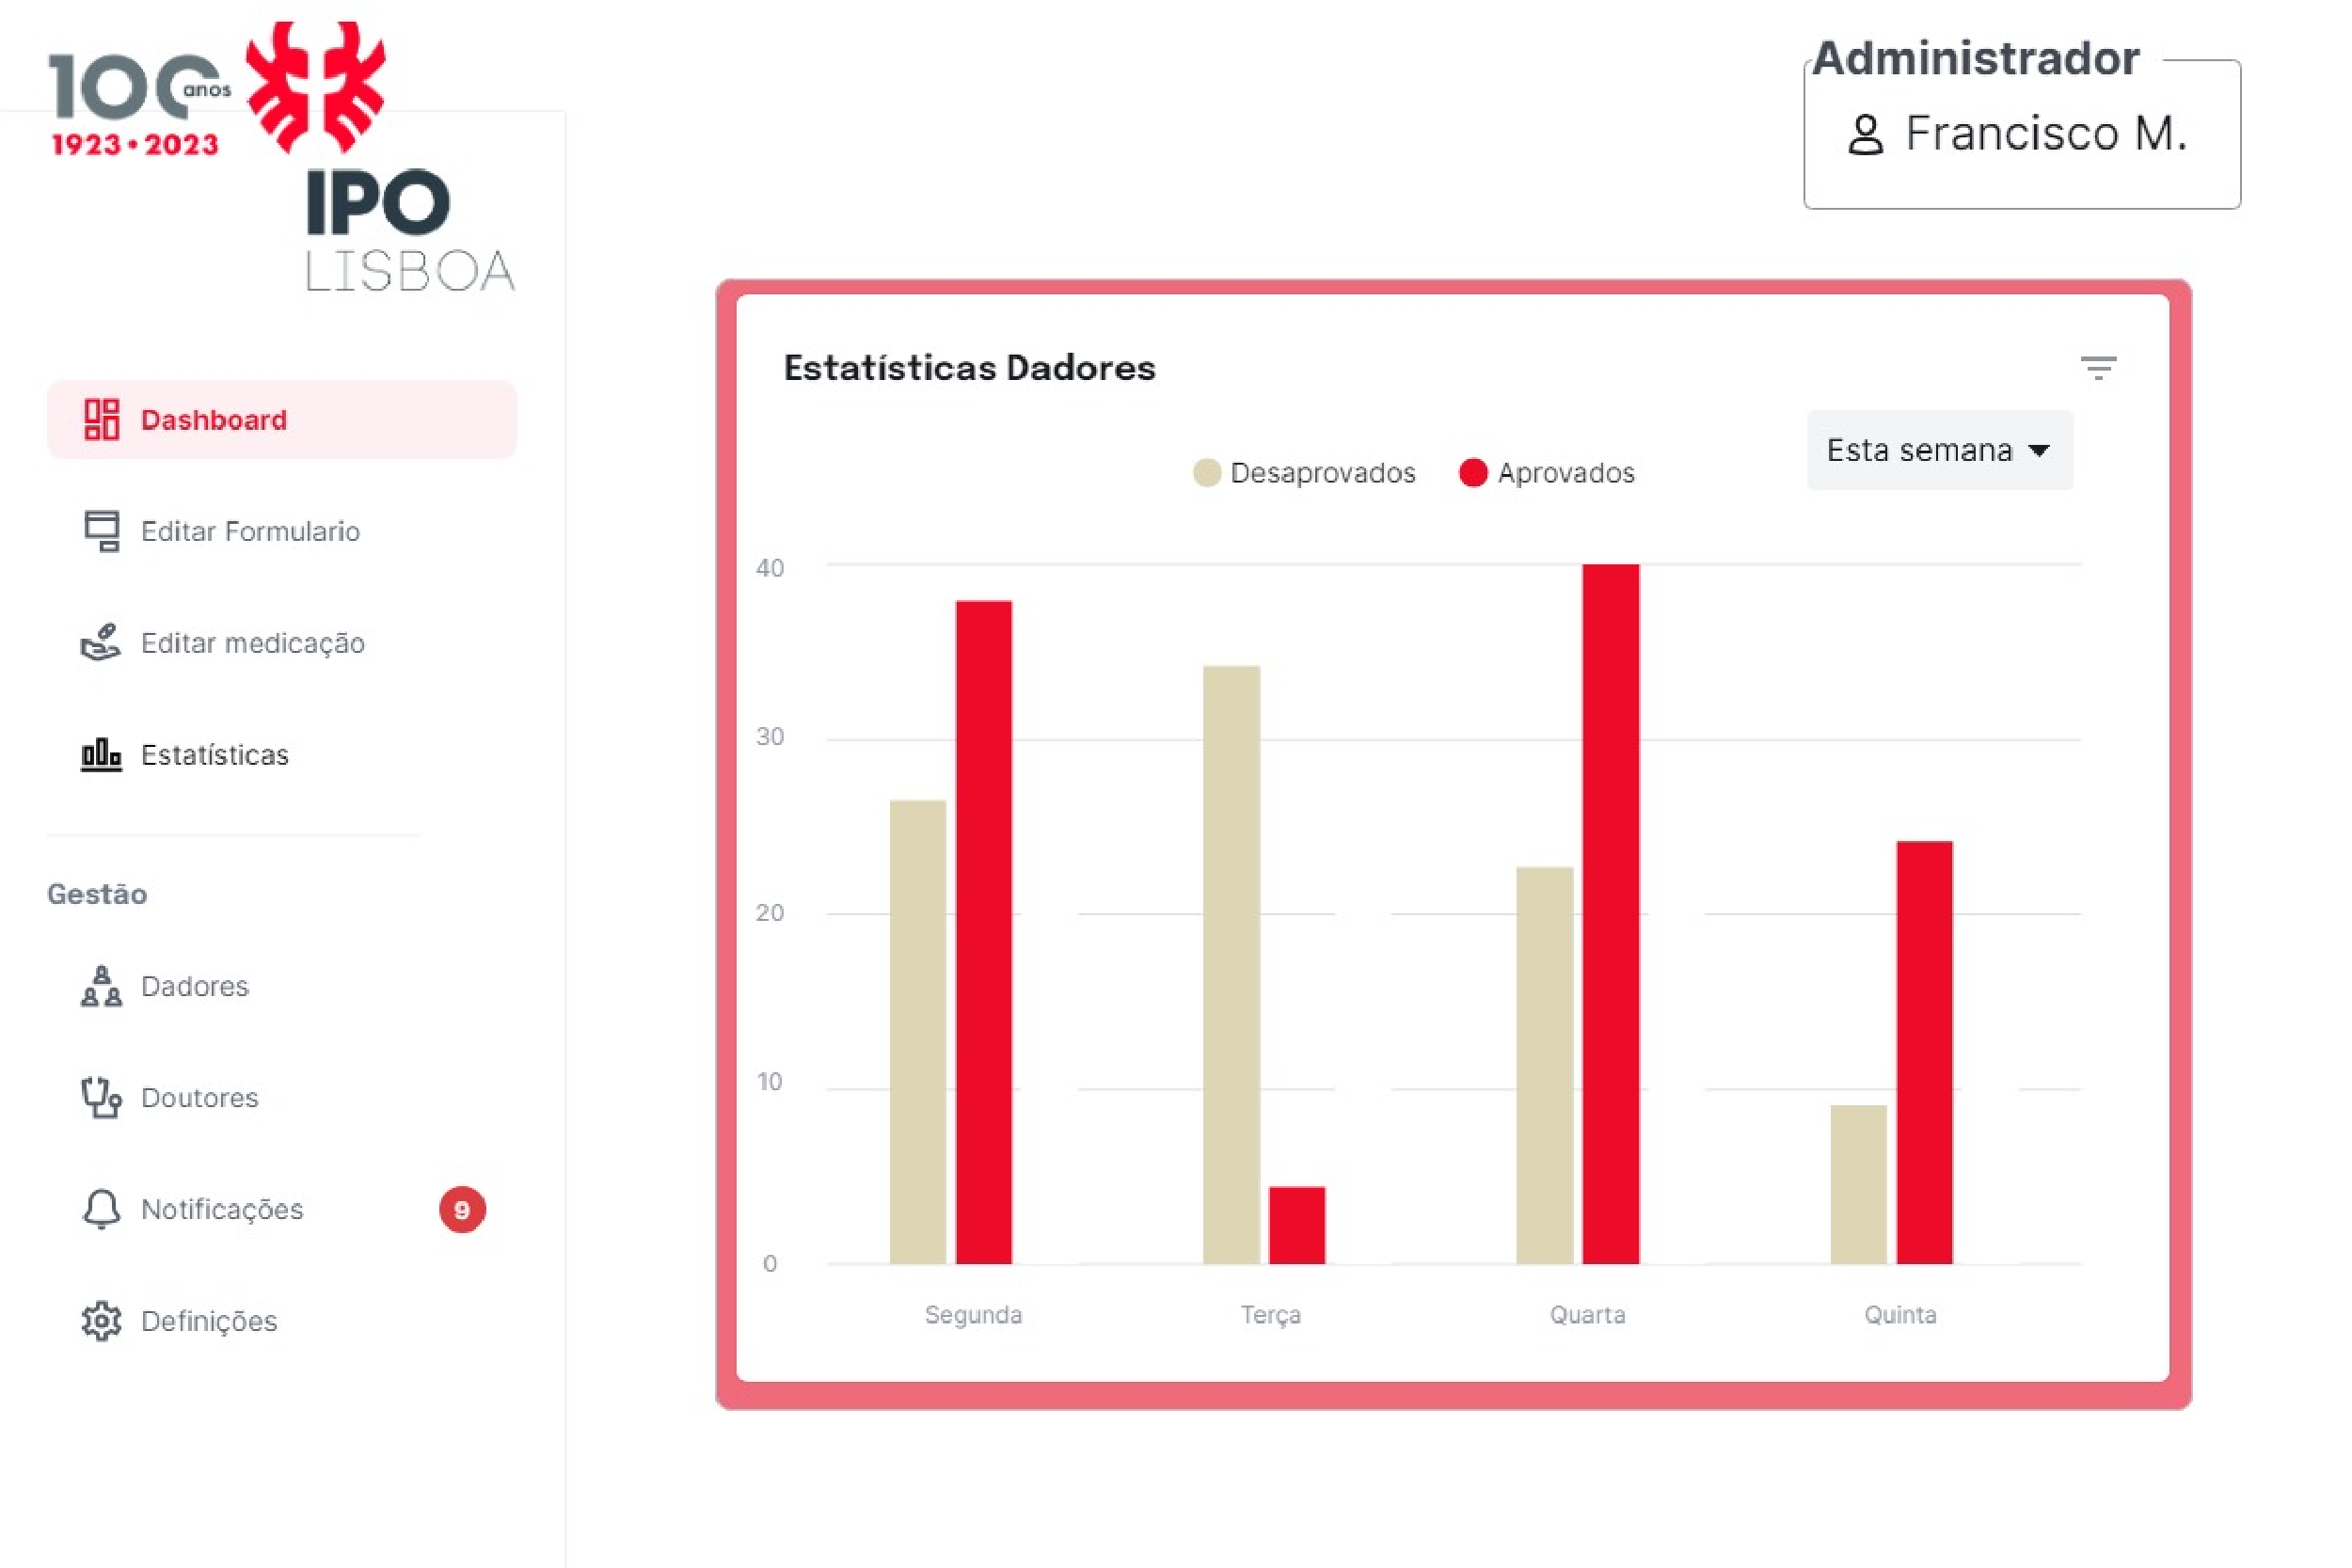
\includegraphics{./figures/Backoffice.pdf}}
	\end{center}
	\caption{Backoffice Page Mock.}\label{fig:backoffice}
\end{figure}




%\subsection{Form Services}
%
%The form service is responsible for managing the form resources.
%Figure ~\ref{fig:form_services} is a diagram that shows the architecture of the form services.
%
%\begin{figure}[htbp]
%	\begin{center}
%		\resizebox{150mm}{!}{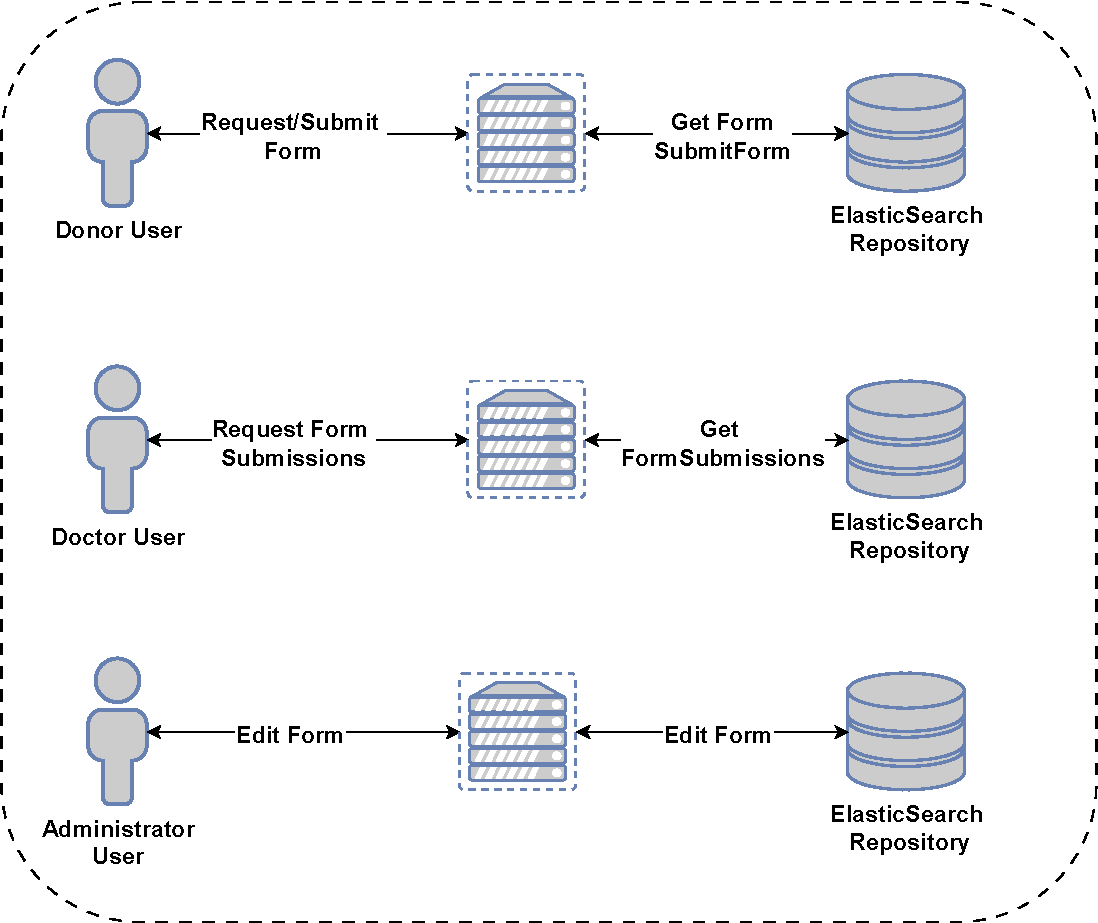
\includegraphics{./figures/formServices.pdf}}
%	\end{center}
%	\caption{Final Form Data Structure.}\label{fig:form_services}
%\end{figure}


% Capitulo 4
\chapter{Exemplos} \label{cap:exemplos}

A nossa solução é apresentada neste capítulo. A solução consiste em grandes ideias, desenvolvidas e testadas.

Exemplo de indentação do segundo parágrafo.

\section{Nome da primeira secção deste capítulo} \label{sec31}
Texto da secção. Seguem-se exemplos de vários parágrafos.

Esta unidade curricular funciona no semestre de Verão de cada ano letivo. Nos casos de impedimento prolongado justificado (designadamente por doença ou por motivos profissionais no caso dos trabalhadores-estudantes), poderá ser prolongada, havendo lugar à elaboração de outro relatório de progresso
e a nova inscrição se o prolongamento for além do período de época especial desse semestre. A entrega da justificação e a sua apreciação deverão ocorrer antes do final do prazo estabelecido para a entrega final.

O estudante só poderá frequentar Projecto e Seminário se, em conjunto com as restantes unidades curriculares em que se inscreve nesse semestre isso corresponder, no máximo, a 44 créditos ECTS, tendo acumulado, pelo menos, 138 créditos. No caso de estudantes em regime de tempo parcial, o valor máximo
está limitado a 30 créditos no ano letivo. Não são admitidas inscrições como unidade curricular isolada.

Anualmente é divulgada a lista de ideias para projetos e respetivos orientadores. Os estudantes poderão propor outras ideias identificando os orientadores. A escolha da ideia de projeto é feita no período de
interrupção letiva após o semestre de Inverno. As propostas de projeto são registadas no início do período letivo do semestre de Verão, verificado que os estudantes reúnem as condições de frequência.
O projeto deve ser realizado em grupo de dois estudantes (excecionalmente um ou três). Cada elemento do grupo tem tarefas específicas pelas quais é responsável. Esta situação deve ficar clara desde o início do projeto.

A orientação dos projetos é feita por docentes da área departamental onde o curso está ancorado ou por especialistas externos, podendo haver coorientadores, mas sendo obrigatória a coorientação por docente da área departamental no caso de orientação externa. O desenvolvimento do projeto é acompanhado de reuniões periódicas do orientador (ou coorientadores) com o grupo. A informação referente ao projeto é mantida em formato eletrónico em local acessível pelos elementos do grupo, pelos orientadores e pelos docentes de Projecto e Seminário.\\

A avaliação de Projecto e Seminário envolve:
\begin{enumerate}
	\item proposta do projeto;
	\item relatório de progresso;
	\item apresentação individual;
	\item cartaz e versão beta do projeto;
	\item relatório de projeto e discussão pública final.
\end{enumerate}

A avaliação incide sobre o trabalho planeado e desenvolvido pelos estudantes, com constrições de tempo e prazos previamente estabelecidos. Se durante a realização do projeto for considerado que este está em risco, ouvidos os estudantes envolvidos, o orientador e o docente da unidade curricular decidem se o projeto continua. Em caso de desistência do estudante, esta deve ser comunicada ao orientador do projeto e ao regente da unidade curricular.

\section{A segunda secção deste capítulo} \label{sec32}
Na segunda secção deste capítulo, vamos abordar o enquadramento,
o contexto e as funcionalidades.

\subsection{A primeira sub-secção desta secção} \label{sec321}
As sub-secções são úteis para mostrar determinados conteúdos de forma
organizada. Contudo, o seu uso excessivo dificulta a leitura do documento.

\subsection{A segunda sub-secção desta secção} \label{sec322}
Esta é a segunda sub-secção desta secção, a qual termina aqui.

\section{Descrição detalhada da solução} \label{sec33}
A solução proposta assenta nas seguintes ideias. O algoritmo~\ref{alg1}
apresenta as ações de pesquisa de um elemento $E$ sobre um grafo $G$.
\begin{algorithm}
\caption{Algoritmo de pesquisa em grafo.}
\label{alg1}
\algorithmicrequire{Grafo G, Elemento E}\\
\algorithmicensure{Localização de E em G}\\
\begin{enumerate}
\item Para todos os vértices $v$ em $G$
\item Pesquisar e obter a localização de $E$
\begin{enumerate}
	\item Iniciar a lista de pontos, $P$
	\item Ordenar $P$
\end{enumerate}	
\end{enumerate}
\end{algorithm}

\newpage
Nalgumas situações, é necessário apresentar excertos de
código que ilustrem aspetos relevantes da implementação.

\begin{verbatim}
namespace ps;
public static void main() {
		System.out.println(``PS - Projecto e Seminário'');
}
\end{verbatim}

% Capitulo 5
\chapter{Testes} \label{cap:testes}

Este é o capítulo de testes. 
É possível forçar a inclusão de todas as referências com \cite{*}.

Modo de matemática em texto $x = ma^2$ e em equação (duas formas):
\[
    x = ma^2
\]

\begin{equation}
    x = ma^2
\end{equation}

% Referências
\bibliographystyle{unsrt}
\bibliography{referencias}
\addcontentsline{toc}{chapter}{Refer\^{e}ncias}

% Apêndices (opcional)
\appendix
%
% Apêndice 1
%
\chapter{Exemplo de apêndice} \label{ap:exemplo}
Este é o primeiro parágrafo do apêndice.


\lipsum[14-16]

\end{document} 